\documentclass{article}

\usepackage{arxiv}

\usepackage[utf8]{inputenc} % allow utf-8 input
\usepackage[T1]{fontenc}    % use 8-bit T1 fonts

% The template loads babel as [english,russian], which makes Russian the main language
% (Russian hyphenation and caption names). This article is in English, so the order is reversed.
\usepackage[russian,english]{babel}
%\usepackage{amsbib}   % in the template; not needed here (the bibliography uses plain \bibitem)
\usepackage[square,sort,comma,numbers]{natbib}
\usepackage{amsfonts}
\usepackage{amssymb}
\usepackage{hyperref}       % hyperlinks
\usepackage{url}            % simple URL typesetting
\usepackage{booktabs}       % professional-quality tables
\usepackage{amsmath}
\usepackage{empheq}
\usepackage{nicefrac}       % compact symbols for 1/2, etc.
\usepackage{microtype}      % microtypography
\usepackage{cleveref}       % smart cross-referencing
\usepackage{graphicx}
\usepackage{subfigure}
\usepackage{doi}
\newtheorem{theorem}{\bf Theorem}
\newtheorem{definition}{\bf Definition}
\newtheorem{lemma}{\bf Lemma}
\newtheorem{corollary}{\bf Corollary}
\newtheorem{proposition}{\bf Proposition}
\usepackage{float}
\usepackage{multirow}
\usepackage{xcolor}
\usepackage{eso-pic}
\newcommand{\arxivstamp}[1]{%
  \AddToShipoutPictureFG{%
    \AtPageLowerLeft{%
      \raisebox{0.26\paperheight}{%
        \hspace{0.03\paperwidth}%
        \rotatebox{90}{%
          \textcolor{gray!85}{\huge #1}%
        }%
      }%
    }%
  }%
}


% main title, then the subtitle on its own line in a smaller size
\title{Multichannel Singular Spectrum Analysis \\ \vspace{1.5mm}
{\Large for Estimating Oscillatory Sources \\ and Localizing Attenuating Oscillations}}

% Here you can change the date presented in the paper title
\date{August 12, 2026}

% the affiliation carries a first-page footnote with the address of Aicumene; both authors share it
\author{ \href{https://orcid.org/0000-0002-8835-6583}{
\includegraphics[scale=0.06]{orcid.pdf}\hspace{1mm}Alexandra Bernadotte} \\
	Aicumene\thanks{Aicumene. \url{https://aicumene.com}}\\
	\texttt{bernadotte@aicumene.com} \\
	\And
	\href{https://orcid.org/0000-0002-9987-4060}{
\includegraphics[scale=0.06]{orcid.pdf}\hspace{1mm}Ivan Menshikov} \\
	Aicumene\footnotemark[1]\\
}

% Uncomment to override  the `A preprint' in the header
%\renewcommand{\headeright}{Technical Report}
%\renewcommand{\undertitle}{Technical Report}
\renewcommand{\shorttitle}{Multichannel Singular Spectrum Analysis}

%%% Add PDF metadata to help others organize their library
\hypersetup{
pdftitle={Multichannel Singular Spectrum Analysis for Estimating Oscillatory Sources and Localizing Attenuating Oscillations},
pdfsubject={cs.HC, eess.SP, q-bio.NC},
pdfauthor={Alexandra Bernadotte, Ivan Menshikov},
pdfkeywords={multichannel singular spectrum analysis, MSSA, Hankel embedding, inverse problem, oscillatory sources, attenuation, source localization, intrinsic oscillatory dimensionality, multichannel time series},
}

\begin{document}
\arxivstamp{AiCumene:2026.044v1 [cs.HC] August 12 2026}
\maketitle

\begin{abstract}
Multichannel time series often arise from a finite number of latent oscillatory sources observed through multiple sensors. A fundamental inverse problem is to determine how many such sources are active and, when a propagation or attenuation model is available, where the sources are located. Previous work by Bernadotte formulated a Hankel-embedding approach to the inverse problem of estimating the number of oscillatory sources in EEG and brain-computer-interface recordings. In that framework, the effective rank of a trajectory embedding provides an estimate of the number of active oscillators. Here we extend this framework from source-number estimation to source-coordinate recovery for attenuating oscillatory systems.

We formulate Multichannel Singular Spectrum Analysis (MSSA) as a block-Hankel method for extracting latent oscillatory modes from multichannel signals. Each channel is embedded into a Hankel trajectory matrix, and all channel-wise embeddings are concatenated into a joint block-Hankel matrix. Singular value decomposition of this matrix separates reproducible lagged multichannel dynamics from residual fluctuations; its signal subspace yields the oscillatory modes, with their frequencies and damping rates, and a spatial loading vector across sensors for every mode. We show that when a latent oscillatory source undergoes distance-dependent amplitude attenuation, the MSSA-derived spatial loading vector is an amplitude fingerprint of the source coordinate, and that without noise it is recovered exactly whenever the sources differ in frequency or damping. If sensor coordinates are known and the attenuation law is known and monotone, source localization reduces to matching this empirical amplitude fingerprint to theoretical attenuation profiles generated by candidate source locations.

The conditions of identifiability are made explicit. The rank of the block-Hankel matrix counts distinct oscillatory modes, so that sources of equal frequency and damping are counted once; they are detected through the phase structure of their common loading and separated by a scan of a two-dimensional subspace, which does not need the statistical independence that blind separation requires. For power-law attenuation, two positions have the same normalized fingerprint exactly when all sensors lie on a sphere with respect to which the positions are mutually inverse, or on a hyperplane in which they are mirror images; $d+2$ sensors in general position therefore determine a source in $\mathbb{R}^d$, and an array on a sphere is unambiguous inside it. For exponential attenuation the corresponding surfaces are hyperboloids. A first-order formula gives the accuracy of the recovered position, and simulations attain it with the number of sources estimated from the data. With a gain matrix in place of the scalar attenuation law the same procedure localizes current dipoles, for which a distance-only model fails. The resulting framework applies to neurophysiology, wearable sensing, industrial monitoring, geophysics, wireless systems, and financial markets, where latent oscillatory regimes may be observed through multiple attenuated channels or indicators.
\end{abstract}


\keywords{Multichannel singular spectrum analysis \and MSSA \and Hankel embedding \and Inverse problem \and Oscillatory sources \and Attenuation \and Source localization \and Intrinsic oscillatory dimensionality \and Multichannel time series}

\section{Introduction}\label{sec:introduction}

Many biological, physical, technological, and economic systems are observed through multichannel time series. In such systems, the measured channels are often mixtures of a smaller number of latent dynamical sources. These sources may be oscillatory, quasi-periodic, transient, damped, amplified, or locally coherent over finite windows. A central problem is therefore inverse: from observed multichannel signals, infer the latent structure that generated them.

Two inverse problems are particularly important. The first is structural: how many latent oscillatory sources are active \cite{ref-BernadotteBuchstaber, ref-Bernadotte05}? The second is geometric: where are these sources located, either in physical space or in an abstract sensor, feature, or factor space?

Previous work by Bernadotte addressed the first inverse problem: estimating the number of oscillatory sources using Hankel embeddings and singular-spectrum analysis \cite{ref-BernadotteBuchstaber, ref-Bernadotte05}. In the paper \emph{Estimating the Number of Sources in EEG with Hankel Embedding for Brain-computer Interface} \cite{ref-Bernadotte05}, the Polyharmonic Brain Signal Model was introduced to justify trajectory embedding and low-rank approximation. Each EEG or MEG trace was mapped to a Hankel matrix, and the effective rank of the unfolding was interpreted as the number of oscillatory components in the ideal noise-free case. The paper proposed an algorithm for evaluating the number of sources, or oscillators, from the singular or eigenvalue spectrum of unfolded data. The approach rests on the theory of the unfolding of time series and its geometry on Grassmann manifolds \cite{ref-Buchstaber, ref-BuchstaberMaslov}. It has since been developed into a classifier of time series \cite{ref-Bernadotte10} and into a marker of brain state, the number of oscillatory modes in a window of EEG \cite{ref-Bernadotte07}.

A related work, \emph{A Lightweight Hankel-Embedded Pipeline for Real-Time EEG Filtering and Classification} \cite{ref-Bernadotte06}, developed a practical Hankel-based pipeline for oscillator extraction, adaptive filtering, jPCA-based dynamics, and lightweight EEG classification. This showed that Hankel-derived oscillatory structures are not only theoretically meaningful but also useful for real-time multichannel signal processing.

The present article extends this line of work. We retain the first result --- that Hankel/MSSA structure can estimate the number of active oscillatory sources --- and add a second result: if oscillatory sources undergo distance-dependent amplitude attenuation, then the spatial loading vector recovered by MSSA becomes an amplitude fingerprint of the source coordinate. Under appropriate identifiability conditions, this fingerprint can be used to recover the coordinates of the sources.

Thus, MSSA is used not only as a decomposition or denoising method, but as a regularizing operator for inverse problems. It first estimates the number of active oscillatory sources and their spatial loadings. Then, using a known attenuation model and known sensor coordinates, these loadings are matched to theoretical source-to-sensor profiles to recover source coordinates.

The paper states both results precisely and tests them.

\begin{enumerate}
\item
  The rank of the block-Hankel matrix equals the number of distinct exponential modes of the recording, whatever the number of channels (Theorem~\ref{thm:rank}). It counts sources when their frequencies or damping rates differ, and counts once those that coincide in both (Corollary~\ref{cor:modes}).
\item
  The spatial loading of a mode is defined through the poles and amplitudes of the signal subspace, and not through individual singular vectors; without noise it is recovered exactly (Theorem~\ref{thm:loadings}). Its phase structure distinguishes a single source from two sources that share a mode (Proposition~\ref{prop:shared-mode}).
\item
  The injectivity of the normalized attenuation map, on which localization depends, is characterized geometrically for power-law and exponential attenuation (Theorems~\ref{thm:power-law} and \ref{thm:exponential}), and the accuracy of the recovered position is given to first order (Proposition~\ref{prop:accuracy}).
\item
  The scalar attenuation law is the simplest case of a forward model with a known gain matrix, which is the form that EEG and MEG require (Section~\ref{sec:forward-models-with-a}).
\item
  Every statement is checked numerically, the complete procedure is run with the number of sources estimated from the data, and the spatial step is compared with blind separation of independent components (Section~\ref{sec:numerical-experiments}).
\end{enumerate}

\subsection{Relation to earlier work}\label{sec:relation-to-earlier-work}

The framework continues our earlier work on the unfolding of time series: the estimation of the number of sources from the rank of a Hankel embedding \cite{ref-BernadotteBuchstaber, ref-Bernadotte05}, the real-time extraction of oscillators \cite{ref-Bernadotte06}, classification by the subspace of the embedding \cite{ref-Bernadotte10}, and the oscillatory dimension of brain states \cite{ref-Bernadotte07}. Singular spectrum analysis, on which it draws, decomposes a series through the singular value decomposition of its trajectory matrix \cite{ref-Broomhead, ref-Vautard, ref-Golyandina01, ref-Golyandina02}; the multichannel form stacks the trajectory matrices of several channels \cite{ref-Golyandina03, ref-Plaut}. Three further bodies of work meet in the second inverse problem.

\emph{Array signal processing.} In \cite{ref-BernadotteBuchstaber, ref-Bernadotte05} the number of sources is read from the rank of the unfolding of the recording. In array processing it is estimated from the eigenvalues of a covariance matrix \cite{ref-Wax, ref-Kritchman}, and the parameters of the sources from its signal subspace: MUSIC scans a manifold of candidate array responses for vectors close to the subspace \cite{ref-Schmidt}, and ESPRIT reads the parameters from a shift invariance \cite{ref-Roy}. In that literature the subspace is spatial, formed from the covariance between sensors, and the manifold is parametrized by the direction of arrival. Here the subspace is temporal --- the trajectory space of the recording --- and space enters afterwards, through the loading of each temporal mode.

\emph{Localization from amplitudes.} The oscillatory components extracted in \cite{ref-Bernadotte06} were used for filtering and classification, and their distribution over the sensors was not interpreted. Locating a source from the energy received at distributed sensors is known as energy-based localization: ratios of energies at pairs of sensors confine the source to hyperspheres, which are intersected by least squares or fitted by maximum likelihood \cite{ref-Li, ref-Sheng, ref-Meng}. Gain ratios of arrival have been combined with time differences of arrival \cite{ref-Ho}, and positioning from received signal strength is standard in wireless sensor networks \cite{ref-Patwari}. The Apollonius and hyperboloid systems of Section~\ref{sec:special-cases-of-attenuation} are the noise-free form of these estimators. Such methods measure the energy of the received signal in a band, so several sources have to be fitted jointly \cite{ref-Sheng}.

\emph{Electromagnetic source imaging.} The source counts of \cite{ref-BernadotteBuchstaber, ref-Bernadotte05} and the oscillatory dimension of \cite{ref-Bernadotte07} say how many generators are active in an EEG, not where they are. In EEG and MEG the forward model is a lead field and localization from a spatial pattern is dipole fitting: spatio-temporal dipole models and MUSIC scans of the lead field \cite{ref-Mosher01}, and the fitting of an equivalent dipole to the scalp map of an independent component \cite{ref-Delorme}.

\emph{Blind separation in space.} The modes counted in \cite{ref-BernadotteBuchstaber, ref-Bernadotte05} are temporal, and sources that share a mode have to be separated in space. Independent component analysis \cite{ref-Comon, ref-Hyvarinen} and second-order blind identification \cite{ref-Belouchrani} do this from the statistics of the mixture, without a forward model; in EEG the maps of the components are then fitted with dipoles \cite{ref-Delorme}. These methods require statistically independent sources, at least as many sensors as sources and, for independent component analysis, non-Gaussian signals. The scan of Section~\ref{sec:two-sources-in-one} uses the forward model in place of independence, and Section~\ref{sec:comparison-with-blind-separation} compares the two.

What the present framework adds is the temporal separation that precedes the spatial fit. Each oscillatory mode, defined by its frequency and damping, receives its own spatial fingerprint; the number of modes is decided by a calibrated test; and sources that overlap in space and in frequency band are fitted one at a time, provided their frequencies or damping rates differ by a fraction of the Fourier resolution. The identifiability analysis of Section~\ref{sec:identifiability} applies to any method that localizes from relative amplitudes, whatever its front end.

\section{Multichannel Singular Spectrum Analysis}\label{sec:multichannel-singular-spectrum-analysis}

The embedding is the unfolding of a time series into a Hankel matrix, on which the source-number method of \cite{ref-BernadotteBuchstaber, ref-Bernadotte05} and the pipeline of \cite{ref-Bernadotte06} are built. This section writes it for several channels at once.

\subsection{Multichannel time series}\label{sec:multichannel-time-series}

Let \[
X = \{x_j(t)\}_{j=1,\,t=1}^{m,\,N} \in \mathbb{R}^{m \times N}
\] be a multichannel time series with $m$ observed channels or sensors and $N$ time samples. The goal of MSSA is to extract reproducible lagged structures from $X$, identify the effective number of structured oscillatory modes, and estimate their spatial loading patterns across the sensors.

\subsection{Channel-wise Hankel embedding}\label{sec:channel-wise-hankel-embedding}

For each channel $x_j(t)$, choose an embedding length $L$ and define $K = N - L + 1$. The Hankel trajectory matrix of channel $j$ is \[
H_L(x_j) =
\begin{bmatrix}
x_j(1) & x_j(2) & \cdots & x_j(K) \\
x_j(2) & x_j(3) & \cdots & x_j(K+1) \\
\vdots & \vdots & \ddots & \vdots \\
x_j(L) & x_j(L+1) & \cdots & x_j(N)
\end{bmatrix}
\in \mathbb{R}^{L \times K}.
\] Each column of $H_L(x_j)$ is a delayed window of the original signal. The channel is therefore transformed from a one-dimensional time series into a trajectory in an $L$-dimensional delay-coordinate space.

\subsection{Block-Hankel MSSA matrix}\label{sec:block-hankel-mssa-matrix}

The multichannel trajectory matrix is obtained by stacking all channel-wise Hankel matrices: \[
\mathcal{H}_L(X) =
\begin{bmatrix}
H_L(x_1) \\ H_L(x_2) \\ \vdots \\ H_L(x_m)
\end{bmatrix}
\in \mathbb{R}^{mL \times K}.
\] This construction preserves time alignment across sensors: the $k$-th column of $\mathcal{H}_L(X)$ contains delayed segments of all channels beginning at the same time.

MSSA differs from independent SSA because the decomposition is performed jointly across sensors. A weak oscillatory source may not be visible in one channel alone, but if it is coherent across several channels, it can appear as a significant component in the block-Hankel spectrum. Appendix~\ref{app:joint-and-channel} gives the size of the effect: an oscillation shared by eight channels at $-17.5$ dB is detected in 96 \% of joint analyses and in 11 \% of single-channel ones. The gain belongs to shared structure only; an oscillation confined to one channel is detected better by that channel alone.

\subsection{Singular value decomposition}\label{sec:singular-value-decomposition}

The MSSA matrix is decomposed as \[
\mathcal{H}_L(X) = U \Sigma V^{\top}, \qquad \Sigma = \operatorname{diag}(\sigma_1, \dots, \sigma_p), \quad \sigma_1 \ge \sigma_2 \ge \dots \ge 0 .
\] The leading singular components represent reproducible lagged multichannel patterns. The singular values measure the strength of these patterns. The lower spectral tail is typically associated with noise, unstructured fluctuations, and residual activity.

The decomposition provides three objects: singular values $\sigma_i$, used to estimate the number of structured modes; temporal components, encoded in $V$; and spatial-lagged loading patterns, encoded in $U$. For inverse source reconstruction, the important object is the spatial loading profile across sensors associated with a recovered latent mode.

Two remarks prepare what follows. The same decomposition is obtained from the eigenvectors of the lagged scatter $\mathcal{H}_L(X)\mathcal{H}_L(X)^{\top}$ of size $mL \times mL$, which is the faster route when $mL \ll K$. And a single singular vector is in general not the pattern of one source: when two sources contribute components of similar strength, the singular vectors are mixtures of both (Sections~\ref{sec:mssa-spatial-loading-as} and \ref{sec:two-sources-of-different}). What the data determine is the subspace spanned by the leading singular vectors.

\section{Oscillatory source model}\label{sec:oscillatory-source-model}

The model is the polyharmonic signal model of \cite{ref-BernadotteBuchstaber, ref-Bernadotte05}: every source is a finite combination of exponentially modulated harmonics. The classifier of \cite{ref-Bernadotte10} rests on the same finite-rank property.

\subsection{Latent oscillatory sources}\label{sec:latent-oscillatory-sources}

Assume that the observed multichannel signal is generated by $r$ latent oscillatory sources $s_1(t), \dots, s_r(t)$. Each source may be represented locally as an exponentially modulated oscillation, \[
s_k(t) = e^{\lambda_k t} \sin(\omega_k t + \phi_k),
\] or, more generally, as a finite combination of exponential atoms. The observed signal at sensor $j$ is 
\begin{equation} \label{eq:model}
x_j(t) = \sum_{k=1}^{r} a_{jk}\, s_k(t) + \varepsilon_j(t),
\end{equation} where $a_{jk}$ is the contribution of source $k$ to sensor $j$, $s_k(t)$ is the temporal signal of source $k$, and $\varepsilon_j(t)$ is noise. In matrix form, \[
X = AS + E,
\] where $A \in \mathbb{R}^{m \times r}$ is the spatial mixing matrix and $S \in \mathbb{R}^{r \times N}$ contains the temporal source signals. The complex number $z_k = e^{\lambda_k + i\omega_k}$ is the pole of source $k$; it carries its frequency and its damping rate.

\subsection{Finite-rank Hankel structure}\label{sec:finite-rank-hankel-structure}

The key mathematical fact is that finite sums of exponential atoms generate finite-rank Hankel matrices. Let \[
x(t) = \sum_{i=1}^{n} c_i z_i^{\,t},
\] where $z_i \in \mathbb{C} \setminus \{0\}$ are distinct and $c_i \neq 0$. Then the Hankel trajectory matrix $H_L(x)$ admits a Vandermonde factorization \[
H_L(x) = V_L(z)\, \operatorname{diag}(c_1 z_1, \dots, c_n z_n)\, V_K(z)^{\top},
\] in which the columns of $V_L(z)$ are the vectors $v_L(z_i) = (1, z_i, \dots, z_i^{L-1})^{\top}$. If $L \ge n$ and $K \ge n$, the Vandermonde matrices have full column rank, so $\operatorname{rank} H_L(x) = n$ \cite{ref-Golyandina01}. A real oscillatory mode corresponds to a complex conjugate pair of exponential atoms. Therefore, $r$ real oscillatory modes generate a Hankel rank of $2r$ in the noise-free case. This justifies the use of SSA/MSSA for estimating the number of active oscillatory sources.

For several channels the statement takes the following form.

\begin{theorem}[Rank of the block-Hankel matrix] \label{thm:rank}
Let every channel be a combination of the same $n$ exponential atoms, $x_j(t) = \sum_{i=1}^{n} c_{ji} z_i^{\,t}$, with pairwise distinct $z_i \in \mathbb{C} \setminus \{0\}$ and non-zero loading vectors $c_i = (c_{1i}, \dots, c_{mi})^{\top}$. If $L \ge n$ and $K \ge n$, then $\operatorname{rank} \mathcal{H}_L(X) = n$ for every number of channels $m$.
\end{theorem}

\textit{Proof.} The entry of $\mathcal{H}_L(X)$ in channel block $j$, row $l$ and column $k$ is $x_j(l + k - 1) = \sum_i c_{ji}\, z_i^{\,l-1} \cdot z_i \cdot z_i^{\,k-1}$, hence \[
\mathcal{H}_L(X) = \sum_{i=1}^{n} z_i\, \bigl(c_i \otimes v_L(z_i)\bigr)\, v_K(z_i)^{\top}.
\] The rank is at most $n$. The vectors $c_i \otimes v_L(z_i)$ are linearly independent: if $\sum_i \beta_i\, c_i \otimes v_L(z_i) = 0$, then $\sum_i \beta_i c_{ji}\, v_L(z_i) = 0$ in every channel $j$; Vandermonde vectors with distinct nodes are independent for $L \ge n$, so $\beta_i c_{ji} = 0$ for all $i$ and $j$, and since every $c_i$ has a non-zero entry, $\beta_i = 0$. The vectors $v_K(z_i)$ are independent for $K \ge n$. $\square$

\begin{corollary}[Modes and sources] \label{cor:modes}
In model \eqref{eq:model} without noise, let the sources have poles $z_k = e^{\lambda_k + i\omega_k}$ with $0 < \omega_k < \pi$. If the $r$ poles are pairwise distinct, $\operatorname{rank} \mathcal{H}_L(X) = 2r$. If several sources share a pole, they contribute a single conjugate pair of atoms between them, and the rank is twice the number of distinct poles (provided that the joint loading of every pole is non-zero).
\end{corollary}

The second part matters in practice. Two sources of the same frequency and damping but of different phase are linearly independent as time series --- $\operatorname{rank} S = r$ holds --- and are nevertheless one mode of the trajectory matrix. Conversely, a source whose waveform is not a single modulated sinusoid, such as a rhythm with harmonics, contributes one mode for each of its components. The quantity recovered by the first inverse problem is therefore the number of distinct oscillatory modes. It is the number of sources when every source is one mode and no two sources share a mode.

In the language of automata the rank is a number of states: a series whose Hankel matrix has rank $n$ is computed by a weighted automaton with $n$ states and by none with fewer \cite{ref-Fliess}. Theorem~\ref{thm:rank} then says that observing the same modes through more channels adds no states. State counts do not always behave so mildly. For the deterministic finite automata that recognize regular languages the number of states can grow exponentially with the length of the regular expression, the exponential explosion problem treated in \cite{ref-BernadotteAutomata}.

\section{First inverse problem: estimating the number of oscillatory sources}\label{sec:first-inverse-problem-estimating}

The first inverse problem is \[
X \longmapsto r .
\] That is, given the observed multichannel signal, estimate the number of active latent oscillatory sources. This problem was previously addressed in Bernadotte's Hankel-embedding framework for EEG/BCI source-number estimation \cite{ref-BernadotteBuchstaber, ref-Bernadotte05}. There, the effective rank or $\varepsilon$-rank of the time-series unfolding was used to infer the number of active oscillatory sources. Since a real oscillatory component contributes two Hankel dimensions, the number of oscillators is estimated as one half of the effective rank.

In MSSA form, define the intrinsic oscillatory dimensionality \cite{ref-Bernadotte07} as 
\begin{equation} \label{eq:dosc}
\widehat{d}_{\mathrm{osc}}(X; L, \tau) = \bigl|\{ i : \sigma_i(\mathcal{H}_L(X)) > \tau \}\bigr|,
\end{equation} where $\tau$ separates structured components from noise. If significant components form conjugate oscillatory pairs, the estimated number of oscillatory sources is \[
\widehat{r} = \tfrac{1}{2}\, \widehat{d}_{\mathrm{osc}} .
\] By Corollary~\ref{cor:modes} this is the number of distinct oscillatory modes, and the number of sources when their poles are distinct.

The threshold decides the result, and two ways of setting it are compared in Section~\ref{sec:the-complete-procedure}.

\emph{Calibrated random-matrix threshold.} Let $\ell_i = \sigma_i^2 / K$ and $\beta = mL/K < 1$. For white noise of variance $\sigma_\varepsilon^2$ and independent entries, the $\ell_i$ of the noise would follow the Marchenko--Pastur law of ratio $\beta$ and the largest of them would converge to $\sigma_\varepsilon^2 (1 + \sqrt{\beta})^2$ \cite{ref-Marchenko, ref-Yin}. The noise variance is estimated by matching the median of the $\ell_i$ to the median of that law, which a few signal components do not disturb, and a component is declared significant when \[
\ell_i > \widehat{\sigma}_\varepsilon^{2}\, (1 + \sqrt{\beta})^{2}\, (1 + \kappa).
\] The correction $\kappa$ is necessary. The largest noise eigenvalue fluctuates about the edge \cite{ref-Johnstone}, and the entries of a trajectory matrix are not independent, every noise sample being repeated along an anti-diagonal \cite{ref-Bryc}; with $\kappa = 0$ the rule reports components in pure white noise in 16--80 \% of trajectory matrices (Appendix~\ref{app:calibration-of-the}). We take for $\kappa$ the 95 \% quantile, over simulated white-noise recordings of the same $m$, $N$ and $L$, of the relative excess of the largest eigenvalue over the edge; this takes under a second and fixes the false-positive rate at 5 \%.

\emph{Surrogate threshold.} A more robust form uses surrogate spectra. Let $X_{\mathrm{sur}}^{(b)}$ be surrogate signals, $b = 1, \dots, B$, obtained by permuting the samples of every channel independently, which destroys all temporal structure and keeps the distribution of amplitudes. For each surrogate, compute singular values $\sigma_i^{(b)} = \sigma_i(\mathcal{H}_L(X_{\mathrm{sur}}^{(b)}))$. Then \[
\widehat{d}_{\mathrm{osc}}(X) = \bigl|\{ i : \sigma_i(\mathcal{H}_L(X)) > Q_{1-\eta}(\sigma_i^{\mathrm{surrogate}}) \}\bigr| ,
\] where $Q_{1-\eta}$ is the quantile of level $1 - \eta$ over the surrogates. This estimates the number of statistically significant lagged oscillatory dimensions.

The two thresholds behave differently. The surrogate spectrum is that of white noise with the total variance of the recording, signal included. It is therefore conservative: with sources of comparable strength it returns the correct number in all trials from $-5$ dB upward, but it masks a weak source beside a strong one --- at an amplitude ratio of ten the weak source is missed in every trial, while the calibrated threshold finds both in 96 \%. Since attenuation makes distant sources weak, we use the calibrated threshold as the default and the surrogate threshold as a check. Both assume a white noise floor. A coloured background is itself a set of large eigenvalues and has to be whitened, or tested against a null that carries its colour \cite{ref-Allen}, before the count is interpreted (Appendix~\ref{app:calibration-of-the}).

Thus, the first inverse problem is solved structurally: \[
X \xrightarrow{\ \mathrm{MSSA}\ } \widehat{d}_{\mathrm{osc}} \longrightarrow \widehat{r}.
\]

\section{Second inverse problem: recovering coordinates of attenuating oscillatory sources}\label{sec:second-inverse-problem-recovering}

We now consider the second inverse problem: \[
X \longmapsto Q = (q_1, \dots, q_r),
\] where $q_k$ are the coordinates of the latent oscillatory sources. The earlier work \cite{ref-BernadotteBuchstaber, ref-Bernadotte05, ref-Bernadotte06} estimated the number of sources and extracted their time courses; their positions were outside its scope.

The key assumption is that the source signal undergoes distance-dependent amplitude attenuation before reaching each sensor. Therefore, different sensors record the same temporal mode with different amplitudes. These amplitudes encode the geometry of the source-sensor configuration. Attenuation here means the decay of amplitude with distance; decay in time is the damping $\lambda_k$ of Section~\ref{sec:latent-oscillatory-sources} and is a property of the source.

\subsection{Forward model with attenuation}\label{sec:forward-model-with-attenuation}

Let sensors have known coordinates $p_1, \dots, p_m \in \mathbb{R}^{d}$. Let the $k$-th source have unknown coordinate $q_k \in \Omega \subset \mathbb{R}^{d}$. Assume that the contribution of source $k$ to sensor $j$ is 
\begin{equation} \label{eq:attenuation}
a_{jk} = \alpha_k\, g(\lVert p_j - q_k \rVert),
\end{equation} where $\alpha_k > 0$ is the intrinsic amplitude of source $k$, $g(\rho)$ is a known attenuation function of the distance $\rho$, and $g$ is typically strictly decreasing. Then the observed signal is \[
x_j(t) = \sum_{k=1}^{r} \alpha_k\, g(\lVert p_j - q_k \rVert)\, s_k(t) + \varepsilon_j(t),
\] or $X = A(Q) S + E$ with $A_{jk}(Q) = \alpha_k\, g(\lVert p_j - q_k \rVert)$. For a position $q$ define the attenuation profile \[
g_q = \bigl(g(\lVert p_1 - q \rVert), \dots, g(\lVert p_m - q \rVert)\bigr)^{\top}.
\] The $k$-th column of $A(Q)$ is $a_k = \alpha_k\, g_{q_k}$. This vector is the amplitude fingerprint of the source coordinate $q_k$.

\subsection{MSSA spatial loading as an amplitude fingerprint}\label{sec:mssa-spatial-loading-as}

After MSSA separates the latent modes, each recovered oscillatory source is associated with a spatial loading vector $\widehat{a}_k = (\widehat{a}_{1k}, \dots, \widehat{a}_{mk})^{\top}$. Under the attenuation model, \[
\widehat{a}_k \approx \alpha_k\, g_{q_k}.
\] Thus, the vector of spatial loadings recovered by MSSA is an empirical amplitude fingerprint of the source coordinate. This is the central bridge between MSSA and the coordinate inverse problem.

The loading has to be defined with some care, because the left singular vectors do not provide it directly. By Theorem~\ref{thm:rank} the leading singular vectors span the same subspace as the vectors $c_i \otimes v_L(z_i)$, but each of them is a combination of these vectors, and when two sources have similar strength the combination mixes them: this is the failure of strong separability known in singular spectrum analysis \cite{ref-Golyandina04}. The subspace, however, determines the poles, and the poles determine the loadings.

Let $U \in \mathbb{R}^{mL \times 2r}$ hold the leading left singular vectors. Let $U^{\uparrow}$ be $U$ without the last row of every channel block and $U^{\downarrow}$ be $U$ without the first row of every channel block.

\begin{theorem}[Recovery of the spatial loadings] \label{thm:loadings}
Let $X = AS$ with sources $s_k(t) = e^{\lambda_k t} \sin(\omega_k t + \phi_k)$ whose poles $z_k = e^{\lambda_k + i\omega_k}$, $0 < \omega_k < \pi$, are pairwise distinct, and let no column of $A$ vanish. If $L \ge 2r + 1$ and $K \ge 2r$, then

\begin{enumerate}
\renewcommand{\labelenumi}{(\roman{enumi})}
\item
  the eigenvalues of $\Phi = (U^{\uparrow})^{+} U^{\downarrow}$ are the $2r$ poles $z_k$ and $\bar{z}_k$;
\item
  the amplitudes $C \in \mathbb{C}^{m \times 2r}$ in $x_j(t) = \sum_i C_{ji} z_i^{\,t}$ are the unique solution of the linear system $X^{\top} = V_N(z)\, C^{\top}$;
\item
  the column $c_k$ of $C$ that belongs to $z_k$ equals $\tfrac{1}{2} e^{i\theta_k} a_k$ with $\theta_k = \phi_k - \pi/2$, so that 
\begin{equation} \label{eq:loading}
a_k = \pm\, 2\, \mathrm{Re}\bigl(e^{-i\theta_k} c_k\bigr), \qquad \theta_k = \tfrac{1}{2} \arg\bigl(c_k^{\top} c_k\bigr) \pmod{\pi}.
\end{equation}
\end{enumerate}

The loading vector of every source is thus recovered exactly up to sign, together with its waveform $s_k(t) = \pm\mathrm{Re}(e^{i\theta_k} z_k^{\,t})$. For a positive attenuation law the sign is fixed by requiring positive entries.
\end{theorem}

\textit{Proof.} (i) By the factorization in the proof of Theorem~\ref{thm:rank}, the columns of $W = [\, c_i \otimes v_L(z_i) \,]_{i=1}^{2r}$ span the column space of $\mathcal{H}_L(X)$, so $U = WT$ with $T$ invertible. Deleting the last row of every block gives $W^{\uparrow} = [\, c_i \otimes v_{L-1}(z_i) \,]$, and deleting the first gives $W^{\downarrow} = W^{\uparrow} D$ with $D = \operatorname{diag}(z_i)$. The matrix $W^{\uparrow}$ has full column rank because $L - 1 \ge 2r$, by the argument of Theorem~\ref{thm:rank}. Hence $U^{\downarrow} = U^{\uparrow}\, T^{-1} D T$, the solution $\Phi = T^{-1} D T$ is unique, and its eigenvalues are the $z_i$. (ii) $V_N(z)$ has full column rank since $N \ge 2r$. (iii) $s_k(t) = \mathrm{Im}(e^{i\phi_k} z_k^{\,t}) = (e^{i\phi_k} z_k^{\,t} - e^{-i\phi_k} \bar{z}_k^{\,t})/(2i)$, so the coefficient of $z_k^{\,t}$ in channel $j$ is $a_{jk}\, e^{i\phi_k}/(2i)$; then $c_k^{\top} c_k = \tfrac{1}{4} e^{2i\theta_k} \lVert a_k \rVert^2$. $\square$

With noise, the same three steps are applied to the estimated subspace: this is the ESPRIT estimator \cite{ref-Roy, ref-Hua} applied to the block-Hankel matrix, followed by linear least squares. Once the poles are fixed the loading is linear in the data, with \[
\operatorname{Var}(\widehat{a}_{jk}) \approx 2\, \sigma_\varepsilon^{2}\, v_k, \qquad v_k = \bigl[(V_N^{\mathsf{H}} V_N)^{-1}\bigr]_{kk},
\] and $v_k \approx 1/N$ for an undamped mode, which is the bound for the amplitude of a sinusoid of unknown frequency \cite{ref-Rife}.

Two properties of this definition are used below. It does not require the modes to be orthogonal or of different strength. And it yields a signed vector: for a positive attenuation law all entries have one sign, while for the forward models of Section~\ref{sec:forward-models-with-a} the signs carry information.

\subsection{Sources that share a mode}\label{sec:sources-that-share-a}

\begin{proposition} \label{prop:shared-mode}
Let sources $k$ and $l$ share a pole, and let no other source have it. The loading of their common mode is $c = \tfrac{1}{2}\,(e^{i\theta_k} a_k + e^{i\theta_l} a_l)$. If $a_k$ and $a_l$ are not collinear and $\theta_k \not\equiv \theta_l \pmod{\pi}$, the real and imaginary parts of $c$ are linearly independent and span the plane of $a_k$ and $a_l$. If $\theta_k \equiv \theta_l \pmod{\pi}$, then $c$ is proportional to the real vector $a_k \pm a_l$, and the two sources cannot be distinguished from one source with that loading.
\end{proposition}

\textit{Proof.} $[\mathrm{Re}\, c,\ \mathrm{Im}\, c] = \tfrac{1}{2}\,[a_k,\ a_l]\, R$ with $R = \begin{bmatrix} \cos\theta_k & \sin\theta_k \\ \cos\theta_l & \sin\theta_l \end{bmatrix}$ and $\det R = \sin(\theta_l - \theta_k)$. $\square$

A single source has an in-phase loading: after removal of the common phase by \eqref{eq:loading}, the quadrature part $b = 2\, \mathrm{Im}(e^{-i\theta} c)$ vanishes. Under noise, the statistic \[
T = \frac{\lVert \widehat{b} \rVert^{2}}{2\, v\, \widehat{\sigma}_\varepsilon^{2}}
\] is distributed approximately as $\chi^2$ with $m - 1$ degrees of freedom when one source underlies the mode, the phase having been fitted. This gives a test: a mode whose $T$ exceeds the quantile of level $1 - \eta$ is not a single attenuated source. Two sources in one mode can be recovered (Section~\ref{sec:two-sources-in-one}). With three or more, only a two-dimensional subspace of the span of their loadings is observed, and they cannot be recovered individually. A propagation delay that differs between sensors would also produce a quadrature part; the model considered here has none, like the quasi-static approximation of electrophysiology.

\subsection{Forward models with a gain matrix}\label{sec:forward-models-with-a}

The scalar law \eqref{eq:attenuation} is the simplest forward model. More generally, let 
\begin{equation} \label{eq:gain}
a_k = G(q_k)\, \vartheta_k,
\end{equation} where $G(q) \in \mathbb{R}^{m \times n_\vartheta}$ is a known gain matrix and $\vartheta_k \in \mathbb{R}^{n_\vartheta}$ collects the unknown linear parameters of the source. Model \eqref{eq:attenuation} is the case $n_\vartheta = 1$, $G(q) = g_q$, $\vartheta = \alpha$. A current dipole in a volume conductor is the case $n_\vartheta = 3$: $\vartheta$ is the dipole moment, and the columns of $G(q)$, the lead field, are the potentials or magnetic fields produced at the sensors by unit dipoles along three axes \cite{ref-Mosher02, ref-Baillet}. In a homogeneous conductor, for instance, the row of $G(q)$ for sensor $j$ is proportional to $(p_j - q)^{\top} / \lVert p_j - q \rVert^{3}$. Such a pattern changes sign across the array, depends on the orientation of the source, and need not be largest at the nearest sensor. A distance-only law cannot represent it (Section~\ref{sec:a-dipolar-source}), and \eqref{eq:gain} is the form in which the framework applies to EEG and MEG.

\section{Coordinate recovery by attenuation-profile matching}\label{sec:coordinate-recovery-by-attenuation}

The oscillatory modes are obtained as in Sections~\ref{sec:multichannel-singular-spectrum-analysis}--\ref{sec:second-inverse-problem-recovering}, by the Hankel-embedding approach of \cite{ref-BernadotteBuchstaber, ref-Bernadotte05, ref-Bernadotte06}. This section adds the step that turns their loadings into coordinates.

\subsection{One source per mode}\label{sec:one-source-per-mode}

If the intrinsic amplitude $\alpha_k$ is unknown, we compare normalized profiles. The coordinate of source $k$ is estimated by 
\begin{equation} \label{eq:matching}
\widehat{q}_k = \arg\max_{q \in \Omega} \frac{\langle \widehat{a}_k, g_q \rangle}{\lVert \widehat{a}_k \rVert\, \lVert g_q \rVert}.
\end{equation} Equivalently, \[
\widehat{q}_k = \arg\min_{q \in \Omega,\ \alpha > 0}\ \sum_{j=1}^{m} \bigl(\widehat{a}_{jk} - \alpha\, g(\lVert p_j - q \rVert)\bigr)^{2}.
\] For fixed $q$, the optimal amplitude is $\widehat{\alpha}(q) = \langle \widehat{a}_k, g_q \rangle / \lVert g_q \rVert^{2}$. Substituting this back gives a pure optimization problem over coordinates, \[
\widehat{q}_k = \arg\min_{q \in \Omega}\ \lVert \widehat{a}_k - \widehat{\alpha}(q)\, g_q \rVert^{2}.
\] This is a finite-dimensional geometric inverse problem. We solve it by a search over a grid in $\Omega$ followed by least-squares refinement.

The value of the optimum is a diagnostic. The residual fraction $1 - \max_q \cos^2(\widehat{a}_k, g_q)$ is the part of the loading that no position explains. A value well above the level expected from noise indicates a wrong attenuation law, a source outside $\Omega$, or two in-phase sources in one mode (Proposition~\ref{prop:shared-mode}).

\subsection{Two sources in one mode}\label{sec:two-sources-in-one}

For a mode that fails the in-phase test, let $W \in \mathbb{R}^{m \times 2}$ be an orthonormal basis of the span of $\widehat{a}$ and $\widehat{b}$. By Proposition~\ref{prop:shared-mode} the fingerprints of both sources lie in this plane, so the sources are among the minima of \[
\mathcal{J}(q) = 1 - \frac{\lVert W^{\top} g_q \rVert^{2}}{\lVert g_q \rVert^{2}} .
\] This is a scan of the kind used in MUSIC \cite{ref-Schmidt}, in a subspace defined by a temporal mode instead of a spatial covariance. The two deepest minima are refined by the joint fit $\min_{q, q'} \lVert (I - \Pi_{[g_q,\, g_{q'}]})\, [\widehat{a}, \widehat{b}] \rVert_F$, where $\Pi$ denotes the orthogonal projector onto the span of the two profiles. Uniqueness requires that no third position have its profile in the plane, which by a count of conditions needs $m \ge d + 3$ sensors in general position.

The same scan applies when the two sources are not sinusoids but narrow-band signals that occupy one band. The loadings of all modes in the band then lie in the plane of the two fingerprints, and $W$ is taken from them jointly, or from the two leading spatial singular vectors of the band-passed recording (Section~\ref{sec:comparison-with-blind-separation}). No assumption about the statistical relation between the sources is involved, beyond their not being proportional.

\subsection{Gain-matrix models}\label{sec:gain-matrix-models}

For model \eqref{eq:gain} the linear parameters are eliminated in the same way as $\alpha$: \[
\widehat{q}_k = \arg\max_{q \in \Omega} \frac{\lVert \Pi_{G(q)}\, \widehat{a}_k \rVert^{2}}{\lVert \widehat{a}_k \rVert^{2}}, \qquad \widehat{\vartheta}_k = G(\widehat{q}_k)^{+}\, \widehat{a}_k ,
\] where $\Pi_{G(q)}$ is the orthogonal projector onto the range of $G(q)$. This is the fit of an equivalent dipole to a spatial map \cite{ref-Mosher01, ref-Delorme}, applied to the map of an oscillatory mode.

\section{Identifiability}\label{sec:identifiability}

In the first inverse problem, identifiability rests on the finite rank of the unfolding \cite{ref-BernadotteBuchstaber, ref-Bernadotte05} (Theorem~\ref{thm:rank}). In the second, it is a property of the attenuation map.

\begin{proposition}[Reduction to the attenuation map] \label{prop:reduction}
Let the observed multichannel signal be generated by \eqref{eq:model} and \eqref{eq:attenuation}, and let the loading vectors $a_k$ of the $r$ sources be recovered, as they are without noise under the conditions of Theorem~\ref{thm:loadings}. If the normalized attenuation map \[
q \mapsto \frac{g_q}{\lVert g_q \rVert}
\] is injective on $\Omega$, then each source coordinate $q_k$ is uniquely recoverable from its MSSA spatial loading vector $a_k$, up to amplitude scaling and permutation of source labels.
\end{proposition}

\textit{Proof.} For source $k$, $a_k = \alpha_k g_{q_k}$, so $a_k / \lVert a_k \rVert = g_{q_k} / \lVert g_{q_k} \rVert$. If another point $q' \in \Omega$ gave the same normalized attenuation profile, then $g_{q'} / \lVert g_{q'} \rVert = g_{q_k} / \lVert g_{q_k} \rVert$ and, by injectivity, $q' = q_k$. Since the ordering and scaling of separated sources are arbitrary, recovery is unique up to permutation of source labels and amplitude scaling. $\square$

The proposition reduces identifiability to a property of the array and of the attenuation law. For the two laws of Section~\ref{sec:known-or-calibrated-attenuation} this property can be stated geometrically.

\begin{theorem}[Power-law attenuation] \label{thm:power-law}
Let $g(\rho) = \rho^{-\gamma}$ with $\gamma > 0$, and let $q \neq q'$ be two points distinct from the sensors. The profiles $g_q$ and $g_{q'}$ are proportional if and only if all sensors lie

\begin{enumerate}
\renewcommand{\labelenumi}{(\alph{enumi})}
\item
  on a sphere with respect to which $q$ and $q'$ are mutually inverse, or
\item
  on the hyperplane with respect to which $q$ and $q'$ are mirror images.
\end{enumerate}

Moreover, the differential of the normalized attenuation map is singular at $q$ if and only if all sensors lie on a sphere or a hyperplane that passes through $q$.
\end{theorem}

\textit{Proof.} Proportionality means $\lVert p_j - q' \rVert = c\, \lVert p_j - q \rVert$ for all $j$ with one constant $c > 0$. For $c = 1$ the locus $\{x : \lVert x - q' \rVert = \lVert x - q \rVert\}$ is the bisecting hyperplane. For $c \neq 1$ it is the sphere of Apollonius, with centre $o = (q' - c^2 q)/(1 - c^2)$ and radius $R = c\, \lVert q - q' \rVert / |1 - c^2|$. Since $q - o = (q - q')/(1 - c^2)$ and $q' - o = c^2 (q - q')/(1 - c^2)$, the points $q$ and $q'$ lie on one ray from $o$ and $\lVert q - o \rVert\, \lVert q' - o \rVert = R^2$: they are inverse with respect to the sphere \cite{ref-Coxeter}. Conversely, if $q'$ is the inverse of $q$ in a sphere of centre $o$ and radius $R$, then $\lVert x - q' \rVert / \lVert x - q \rVert = R / \lVert q - o \rVert$ for every $x$ on the sphere. For the last statement, the differential annihilates a direction $v$ exactly when $(\partial g_q / \partial q)\, v$ is proportional to $g_q$, that is, when $(q - p_j)^{\top} v = c\, \lVert q - p_j \rVert^{2}$ for all $j$. For $c \neq 0$ this places the sensors on the sphere through $q$ with centre $q - v/(2c)$; for $c = 0$, on the hyperplane through $q$ orthogonal to $v$. $\square$

\begin{corollary} \label{cor:sensors}
For power-law attenuation and unknown source amplitude:

\begin{enumerate}
\renewcommand{\labelenumi}{(\roman{enumi})}
\item
  if the sensors lie neither on a common sphere nor on a common hyperplane --- which requires $m \ge d + 2$ and holds for $d + 2$ sensors in general position --- the normalized attenuation map is injective on $\mathbb{R}^{d}$ without the sensors, and its differential is nowhere singular;
\item
  $m = d + 1$ affinely independent sensors always lie on their circumscribed sphere, and every source other than the centre of that sphere has exactly one twin, its inverse in the sphere;
\item
  sensors on a sphere $\Sigma$ that do not lie in a hyperplane confuse a point only with its inverse in $\Sigma$; the map is injective inside $\Sigma$ and outside it, so restricting $\Omega$ to the interior, when the sources are known to lie inside the array, removes the ambiguity;
\item
  sensors that span a hyperplane and do not lie on a sphere confuse a point only with its mirror image, and restricting $\Omega$ to one side removes the ambiguity. The mirror ambiguity of a planar array holds for every attenuation law, since all distances coincide.
\end{enumerate}
\end{corollary}

\begin{theorem}[Exponential attenuation] \label{thm:exponential}
Let $g(\rho) = e^{-\mu\rho}$ with $\mu > 0$, and $q \neq q'$. The profiles $g_q$ and $g_{q'}$ are proportional if and only if the difference of distances $\lVert p_j - q' \rVert - \lVert p_j - q \rVert$ is the same number $\Delta$ for all sensors; that is, if and only if all sensors lie on the bisecting hyperplane of $q$ and $q'$ ($\Delta = 0$), on one sheet of a hyperboloid of revolution with foci $q$ and $q'$ ($0 < |\Delta| < \lVert q - q' \rVert$), or on the line through $q$ and $q'$ beyond one of the two points ($|\Delta| = \lVert q - q' \rVert$).
\end{theorem}

\textit{Proof.} $e^{-\mu \rho_j'} = c\, e^{-\mu \rho_j}$ for all $j$ is equivalent to $\rho_j' - \rho_j = -\mu^{-1} \log c$, and $|\Delta| \le \lVert q - q' \rVert$ by the triangle inequality. $\square$

The situation is that of hyperbolic positioning from time differences of arrival \cite{ref-Chan, ref-Torrieri}, with logarithms of amplitude ratios in place of range differences. A second solution is described by $q'$ and $\Delta$, which are $d + 1$ numbers, against $m$ conditions: $d + 1$ sensors may admit one, and $d + 2$ sensors in general position do not. For a general strictly monotone law the same count applies. The normalized fingerprint has $m - 1$ degrees of freedom and the position has $d$, so $m \ge d + 1$ sensors are necessary for a locally unique solution, and one sensor more is what excludes isolated second solutions.

\begin{proposition}[Local identifiability and first-order accuracy] \label{prop:accuracy}
Let $J(q) = \partial g_q / \partial q \in \mathbb{R}^{m \times d}$, with rows $g'(\rho_j)\,(q - p_j)^{\top} / \rho_j$, $\rho_j = \lVert p_j - q \rVert$, and let $\Pi_q^{\perp} = I - g_q g_q^{\top} / \lVert g_q \rVert^{2}$.

\begin{enumerate}
\renewcommand{\labelenumi}{(\alph{enumi})}
\item
  If $\Pi_q^{\perp} J(q)$ has rank $d$, the normalized attenuation map is locally injective at $q$. This requires $m \ge d + 1$.
\item
  If $\widehat{a} = \alpha g_q + e$ with $\mathbb{E}\, e = 0$ and $\operatorname{Cov} e = \sigma_a^{2} I$, the estimate \eqref{eq:matching} satisfies, to first order in $e$, 
\begin{equation} \label{eq:accuracy}
\operatorname{Cov}(\widehat{q}) = \frac{\sigma_a^{2}}{\alpha^{2}}\, \bigl(J^{\top} \Pi_q^{\perp} J\bigr)^{-1}.
\end{equation}
\end{enumerate}
\end{proposition}

\textit{Proof.} (a) The differential of $q \mapsto g_q / \lVert g_q \rVert$ is $\Pi_q^{\perp} J / \lVert g_q \rVert$. (b) The Jacobian of the residual $\widehat{a} - \alpha g_q$ with respect to $(q, \alpha)$ is $-[\alpha J,\ g_q]$. The covariance of the least-squares estimate is $\sigma_a^{2}$ times the inverse of its Gram matrix, whose block for $q$ is $(\alpha^{2} J^{\top} \Pi_q^{\perp} J)^{-1}$ by the Schur complement. $\square$

For an undamped mode in white noise, $\sigma_a^{2} = 2\sigma_\varepsilon^{2}/N$ (Section~\ref{sec:mssa-spatial-loading-as}), and the root-mean-square position error is \[
\mathrm{RMS}(\widehat{q}) = \frac{\sigma_\varepsilon}{\alpha} \sqrt{\frac{2}{N}}\ \mathcal{D}(q), \qquad \mathcal{D}(q) = \Bigl[\operatorname{tr}\bigl(J^{\top} \Pi_q^{\perp} J\bigr)^{-1}\Bigr]^{1/2}.
\] The factor $\mathcal{D}(q)$ depends only on the array and on the law. It plays the part of the geometric dilution of precision of positioning systems \cite{ref-Torrieri}, and it is infinite exactly where the differential of the normalized map is singular. Fig.~\ref{fig:accuracy}c maps it for a grid of nine sensors.

\section{Conditions required for coordinate recovery}\label{sec:conditions-required-for-coordinate}

The inverse problem is solvable under the following conditions. They add to the condition under which the number of sources is read from the rank of the unfolding \cite{ref-BernadotteBuchstaber, ref-Bernadotte05}: that the sources be finite combinations of exponential atoms, observed against a noise floor from which they can be separated.

\subsection{Known sensor coordinates}\label{sec:known-sensor-coordinates}

The sensor coordinates $p_1, \dots, p_m$ must be known. Without sensor geometry, the attenuation profile cannot be mapped to physical or abstract coordinates.

\subsection{Known or calibrated attenuation law}\label{sec:known-or-calibrated-attenuation}

The function $g(\rho)$ must be known or estimated from calibration data. Typical examples include \[
g(\rho) = \frac{1}{\rho^{\gamma}}, \quad \gamma > 0, \qquad \text{or} \qquad g(\rho) = e^{-\mu\rho}, \quad \mu > 0 .
\] More complex attenuation laws are possible, including anisotropic or medium-dependent models, and the gain-matrix models of Section~\ref{sec:forward-models-with-a}. A parameter of the law can also be estimated from the fingerprint itself, together with the position, when the number of sensors allows one more unknown: Section~\ref{sec:sensors-and-the-attenuation} does this for the exponent $\gamma$.

\subsection{Monotonicity of attenuation}\label{sec:monotonicity-of-attenuation}

The attenuation law must be monotone over the relevant distance range: $g'(\rho) < 0$. This ensures that different distances produce different amplitudes. If $g$ is not injective over the relevant range, distance cannot be inferred from amplitude. Monotonicity concerns one sensor. It does not by itself make the normalized attenuation map injective, which is a property of the law and of the array together.

\subsection{Non-degenerate sensor geometry}\label{sec:non-degenerate-sensor-geometry}

The sensor configuration must not create unresolved symmetries. If the source amplitude were known, each sensor would give a distance, and $d + 1$ affinely independent sensors would determine the position; in $\mathbb{R}^{3}$ this means four non-coplanar sensors. When the source amplitude is unknown and only relative amplitudes are available --- the case considered here --- one more sensor is required. For power-law attenuation, $d + 1$ sensors always leave two solutions, and $d + 2$ sensors that lie neither on a sphere nor on a hyperplane give a unique one (Corollary~\ref{cor:sensors}); arrays on a sphere or in a plane are unambiguous once $\Omega$ is restricted to the interior of the sphere or to one side of the plane. For exponential attenuation the surfaces are hyperboloids: $d + 1$ sensors may leave a second solution, and $d + 2$ sensors in general position do not (Theorem~\ref{thm:exponential}). In practice, one uses $m > d + 2$ sensors and solves an overdetermined least-squares problem, whose accuracy is given by \eqref{eq:accuracy}.

\subsection{Injectivity of the normalized attenuation map}\label{sec:injectivity-of-the-normalized}

The essential condition is \[
q \neq q' \quad \Longrightarrow \quad \frac{g_q}{\lVert g_q \rVert} \neq \frac{g_{q'}}{\lVert g_{q'} \rVert}.
\] Equivalently, different coordinates must generate different normalized amplitude fingerprints. If two points produce proportional attenuation profiles, $g_q = c\, g_{q'}$, then they cannot be distinguished when source amplitude is unknown. Section~\ref{sec:identifiability} states when this happens.

\subsection{Temporal separability of sources}\label{sec:temporal-separability-of-sources}

MSSA must be able to separate the temporal source signals. The condition for this is that the poles of the sources be pairwise distinct: the sources must differ in frequency or in damping (Theorem~\ref{thm:loadings}). Linear independence of the source signals, $\operatorname{rank} S = r$, is not sufficient: two sources of one frequency and damping with different phases are independent and still form a single mode. If two sources have identical temporal dynamics up to a factor, $s_1(t) = c\, s_2(t)$, then they appear as a single effective source, \[
a_1 s_1(t) + a_2 s_2(t) = (c\, a_1 + a_2)\, s_2(t),
\] and their individual coordinates cannot be recovered. Between these cases lie two sources that share a pole and differ in phase; they are detected and localized through the plane spanned by their loadings (Sections~\ref{sec:sources-that-share-a} and \ref{sec:two-sources-in-one}).

\subsection{Spatial distinguishability of sources}\label{sec:spatial-distinguishability-of-sources}

Sources with well-separated poles need not have distinct fingerprints: each mode is fitted on its own, and two such sources at one position are both localized there (Section~\ref{sec:two-sources-of-different}). Distinct fingerprints, \[
\frac{g_{q_k}}{\lVert g_{q_k} \rVert} \neq \frac{g_{q_l}}{\lVert g_{q_l} \rVert}, \qquad k \neq l,
\] are required in two situations: for sources that share a mode, and for sources whose frequencies differ by less than about half the Fourier resolution, which are separated only because their loadings differ. For stable recovery in these situations, a stronger separation condition is required, $\angle(g_{q_k}, g_{q_l}) > \delta > 0$. If two such sources are too close, their spatial loadings become nearly collinear and the inverse problem becomes ill-conditioned.

\subsection{Sufficient signal-to-noise ratio}\label{sec:sufficient-signal-to-noise}

In real data, $X = A(Q)S + E$. The recovery is stable only if the structured components are separated from noise in the MSSA spectrum. A practical condition is the existence of a singular-value gap, \[
\sigma_{\widehat{d}_{\mathrm{osc}}} \gg \sigma_{\widehat{d}_{\mathrm{osc}} + 1},
\] which the test of Section~\ref{sec:first-inverse-problem-estimating} turns into a decision with a stated error rate. More formally, perturbation results imply that the recovered subspace is stable when the noise norm is small relative to the spectral gap. Once the modes are detected, the position error is proportional to the noise level and to the dilution factor of the array, by \eqref{eq:accuracy}.

\section{Special cases of attenuation-based localization}\label{sec:special-cases-of-attenuation}

In both cases below the loadings $a_{jk}$ are those of the oscillatory modes of Section~\ref{sec:mssa-spatial-loading-as}, extracted by the Hankel-embedding approach of \cite{ref-BernadotteBuchstaber, ref-Bernadotte05, ref-Bernadotte06}.

\subsection{Power-law attenuation}\label{sec:power-law-attenuation}

Suppose $g(\rho) = \rho^{-\gamma}$. Then $a_{jk} = \alpha_k / \lVert p_j - q_k \rVert^{\gamma}$. Taking ratios eliminates $\alpha_k$: \[
\frac{a_{jk}}{a_{1k}} = \left( \frac{\lVert p_1 - q_k \rVert}{\lVert p_j - q_k \rVert} \right)^{\gamma}.
\] Define $\rho_j = (a_{1k} / a_{jk})^{1/\gamma}$. Then $\lVert p_j - q_k \rVert = \rho_j \lVert p_1 - q_k \rVert$. This gives a system of Apollonius sphere equations: \[
\lVert p_j - q_k \rVert^{2} = \rho_j^{2}\, \lVert p_1 - q_k \rVert^{2}.
\] The source coordinate is recovered from the intersection of these surfaces, or in the noisy case by least squares.

With $p_1$ taken as the origin and $w = \lVert q_k \rVert^{2}$, the equations are linear in $(q_k, w)$: \[
\lVert p_j \rVert^{2} - 2\, p_j^{\top} q_k + (1 - \rho_j^{2})\, w = 0, \qquad j = 2, \dots, m .
\] For $m \ge d + 2$ sensors in general position the $m - 1$ equations determine the $d + 1$ unknowns, and the solution satisfies $w = \lVert q_k \rVert^{2}$ by itself. This closed form is exact without noise and can start the least-squares refinement. For $m = d + 1$ the solutions form a line, and the constraint $w = \lVert q_k \rVert^{2}$ selects the two points of Corollary~\ref{cor:sensors}(ii).

\subsection{Exponential attenuation}\label{sec:exponential-attenuation}

Suppose $g(\rho) = e^{-\mu\rho}$. Then $a_{jk} = \alpha_k e^{-\mu \lVert p_j - q_k \rVert}$. Taking logarithmic ratios, \[
\log \frac{a_{jk}}{a_{1k}} = -\mu\, \bigl( \lVert p_j - q_k \rVert - \lVert p_1 - q_k \rVert \bigr).
\] Thus, \[
\lVert p_j - q_k \rVert - \lVert p_1 - q_k \rVert = -\frac{1}{\mu} \log \frac{a_{jk}}{a_{1k}} =: \Delta_j .
\] This is a system of hyperboloid equations, analogous to time-difference localization, but based on amplitude attenuation rather than arrival time. With $p_1$ as the origin and $R = \lVert q_k \rVert$, squaring $\lVert p_j - q_k \rVert = R + \Delta_j$ gives the linear system \[
-2\, p_j^{\top} q_k - 2\, \Delta_j R = \Delta_j^{2} - \lVert p_j \rVert^{2}, \qquad j = 2, \dots, m,
\] the closed form used in hyperbolic positioning \cite{ref-Chan}.

\section{MSSA-assisted inverse localization algorithm}\label{sec:mssa-assisted-inverse-localization}

Steps 1--3 are the source-number algorithm of \cite{ref-BernadotteBuchstaber, ref-Bernadotte05} in multichannel form, and the extraction of oscillatory modes in Step 4 continues the pipeline of \cite{ref-Bernadotte06}. Steps 5--7 are new.

\textbf{Input:} multichannel signal $X \in \mathbb{R}^{m \times N}$; sensor coordinates $p_1, \dots, p_m$; attenuation function $g(\rho)$ or gain matrix $G(q)$; embedding length $L$; level $\eta$ of the tests; candidate source domain $\Omega$.

\textbf{Step 1. Construct the block-Hankel MSSA matrix} $\mathcal{H}_L(X)$ of Section~\ref{sec:block-hankel-mssa-matrix}.

\textbf{Step 2. Compute the decomposition} $\mathcal{H}_L(X) = U \Sigma V^{\top}$, through the SVD or through the eigenvectors of the lagged scatter.

\textbf{Step 3. Estimate the number of active oscillatory dimensions} $\widehat{d}_{\mathrm{osc}}$ with the calibrated threshold of Section~\ref{sec:first-inverse-problem-estimating}, or with the surrogate threshold.

\textbf{Step 4. Estimate the poles.} With $U$ the first $\widehat{d}_{\mathrm{osc}}$ left singular vectors, compute $\Phi = (U^{\uparrow})^{+} U^{\downarrow}$ and its eigenvalues $\widehat{z}_i$. The modes are the poles with positive frequency; their number is $\widehat{r}$, equal to $\tfrac{1}{2} \widehat{d}_{\mathrm{osc}}$ if components are paired.

\textbf{Step 5. Extract MSSA spatial loadings.} Solve $X^{\top} = V_N(\widehat{z})\, C^{\top}$ by least squares. For each mode $k$ compute the common phase and the loading by \eqref{eq:loading}, \[
\widehat{a}_k = (\widehat{a}_{1k}, \dots, \widehat{a}_{mk})^{\top},
\] its quadrature part $\widehat{b}_k$, and the statistic $T_k$ of Section~\ref{sec:sources-that-share-a}.

\textbf{Step 6. Match the loading to attenuation profiles.} For a mode that passes the in-phase test, compute $g_q$ for candidate coordinates $q \in \Omega$ and estimate \[
\widehat{q}_k = \arg\max_{q \in \Omega} \frac{\langle \widehat{a}_k, g_q \rangle}{\lVert \widehat{a}_k \rVert\, \lVert g_q \rVert}.
\] For a mode that fails it, scan the plane of $\widehat{a}_k$ and $\widehat{b}_k$ for two sources (Section~\ref{sec:two-sources-in-one}). For a gain-matrix model use the projector of Section~\ref{sec:gain-matrix-models}.

\textbf{Step 7. Estimate amplitude and accuracy.} Once $\widehat{q}_k$ is obtained, \[
\widehat{\alpha}_k = \frac{\langle \widehat{a}_k, g_{\widehat{q}_k} \rangle}{\lVert g_{\widehat{q}_k} \rVert^{2}},
\] the residual fraction of Section~\ref{sec:one-source-per-mode} measures the quality of the fit, and \eqref{eq:accuracy} with $\sigma_a^{2} = 2 \widehat{\sigma}_\varepsilon^{2} v_k$ gives the covariance of the position.

\textbf{Output:} $\{\widehat{q}_k, \widehat{\alpha}_k, \widehat{s}_k(t)\}_{k=1}^{\widehat{r}}$ with $\widehat{s}_k(t) = \mathrm{Re}(e^{i\widehat{\theta}_k} \widehat{z}_k^{\,t})$, together with the frequency and damping of every source and the diagnostics of Steps 5 and 7.

\section{Numerical experiments}\label{sec:numerical-experiments}

The number of sources was evaluated on recordings of a non-invasive brain-computer interface in \cite{ref-BernadotteBuchstaber, ref-Bernadotte05}, and the Hankel-embedded pipeline on EEG classification in \cite{ref-Bernadotte06}. The positions of sources are not known in such recordings, so the experiments of this section are simulations.

\subsection{Setting}\label{sec:setting}

Unless stated otherwise, nine sensors form a $3 \times 3$ grid on the unit square ($d = 2$), so that lengths are in units of the side of the array. The sampling rate is 100 Hz, $N = 500$ (five seconds) and $L = 40$. Sources are undamped sinusoids of random phase at random positions in $[0.1, 0.9]^2$, at least 0.12 from every sensor. The attenuation law is $g(\rho) = \rho^{-1}$, or $e^{-3\rho}$ where indicated. Sensor noise is white, Gaussian and of equal variance $\sigma_\varepsilon^{2}$ in all channels. The signal-to-noise ratio is defined at the reference distance $\rho_0 = 0.5$, \[
\mathrm{SNR}_0 = \frac{\alpha^{2}\, g(\rho_0)^{2}}{2\, \sigma_\varepsilon^{2}},
\] the ratio that a source of amplitude $\alpha$ has at a sensor half an array side away. Position errors above 0.1 are called gross. Each point is the result of 300 trials unless noted. In Sections~\ref{sec:one-source}--\ref{sec:a-dipolar-source} the rank is given, so that the localization step is tested separately; in Section~\ref{sec:the-complete-procedure} it is estimated.

\subsection{The exact statements}\label{sec:the-exact-statements}

Without noise the statements of Sections~\ref{sec:oscillatory-source-model}--\ref{sec:special-cases-of-attenuation} hold to machine precision.

\emph{Rank.} Three sources at 8, 11 and 15 Hz give rank 6. When two of them have 8 Hz with different phases the rank is 4, although $\operatorname{rank} S = 3$; when they have 8 Hz with different damping the rank is 6 again (Corollary~\ref{cor:modes}).

\emph{Loadings.} For two sources at 10 and 13 Hz, the loadings of Theorem~\ref{thm:loadings} coincide with the true fingerprints to $1 - \cos < 5 \times 10^{-16}$ at every ratio of source strengths. The energy profiles of pairs of singular vectors deviate by $1 - \cos = 0.05$ (median) at equal strength, by 0.017 at a ratio of 1.05 and by $2 \times 10^{-4}$ at a ratio of 1.5.

\emph{Ambiguities} (Fig.~\ref{fig:ambiguity}). With eight sensors on a circle and a power law, the profiles of a point and of its inverse in the circle coincide to $10^{-16}$ for $\gamma = 0.5$, 1 and 2, and differ for the exponential law. With three sensors the twin is the inverse in the circumscribed circle. With sensors on a line it is the mirror image, for both laws. With the grid of nine sensors there is no twin. For the exponential law and three sensors in the plane a second exact solution exists for 6 of 200 source positions, and for none with four sensors. In three dimensions a point inside a sphere of twelve sensors and its inverse have the same profile to $10^{-16}$. The differential of the normalized map has a smallest singular value of $10^{-16}$ when the sensors lie on a circle or on a line through the source, and of order one otherwise (Theorem~\ref{thm:power-law}).

\emph{Shared mode.} For two sources at 10 Hz in quadrature, the plane spanned by the real and imaginary parts of the loading contains both fingerprints to $10^{-15}$, and the scan of Section~\ref{sec:two-sources-in-one} returns both positions to $10^{-10}$ in 100 of 100 configurations; matching the modulus of the loading to a single profile gives a position 0.12 away from either source (median).

\emph{Closed forms.} The linear systems of Section~\ref{sec:special-cases-of-attenuation} return the position to $10^{-13}$.

\begin{figure}[tb]
\renewcommand{\figurename}{Fig.}
    \centering
    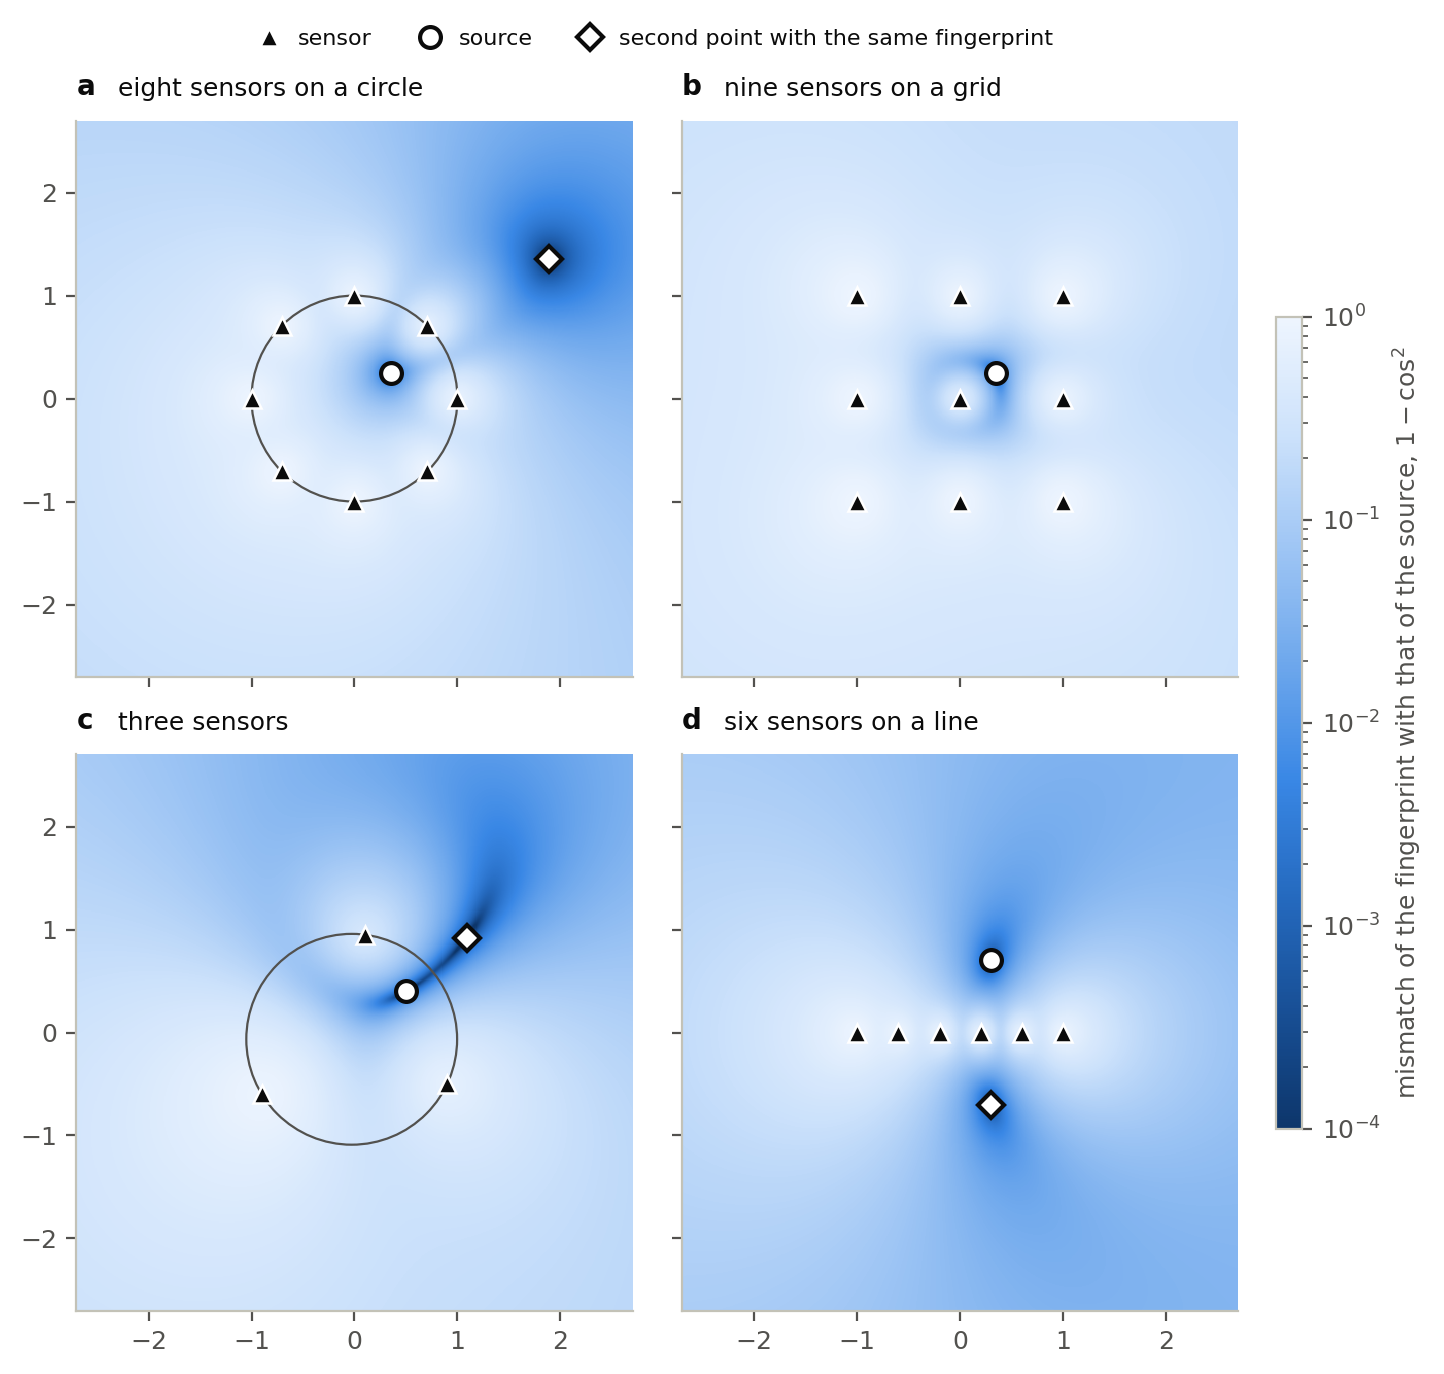
\includegraphics[width=0.82\textwidth]{fig1_ambiguity.png}
    \caption{Where the fingerprint is ambiguous: mismatch $1 - \cos^2$ between the attenuation profile of each point of the plane and that of the source, for power-law attenuation. (a) Sensors on a circle: the inverse of the source in the circle has the same normalized fingerprint. (b) Sensors on a grid: no second point. (c) Three sensors: the twin is the inverse in the circumscribed circle. (d) Sensors on a line: the mirror image.}
    \label{fig:ambiguity}
\end{figure}

\subsection{One source}\label{sec:one-source}

Table~\ref{tab:one-source} and Fig.~\ref{fig:accuracy}a, b give the position error for four ways of obtaining the fingerprint: the signed loading of Theorem~\ref{thm:loadings}, its modulus, the energy of the leading pair of singular vectors in every channel block, and the amplitude from the power in a band of $\pm 1$ Hz around the true frequency, which the other three do not know.

\begin{table}[htb]
\centering
\caption{One source, power law: RMS position error.}
\label{tab:one-source}
\begin{tabular}{l c c c c c}
\toprule
SNR$_0$ (dB) & signed loading & modulus & singular pair & band power & prediction \eqref{eq:accuracy} \\
\midrule
$-15$ & 0.084 & 0.083 & 0.084 & 0.107 & 0.067 \\
$-10$ & 0.041 & 0.042 & 0.044 & 0.050 & 0.038 \\
$0$ & 0.012 & 0.012 & 0.012 & 0.013 & 0.012 \\
$10$ & 0.0039 & 0.0039 & 0.0041 & 0.0040 & 0.0038 \\
$20$ & 0.0011 & 0.0011 & 0.0012 & 0.0012 & 0.0012 \\
\bottomrule
\end{tabular}
\end{table}

From $-10$ dB upward the error follows the first-order prediction within 10 \%, for both laws. Below $-15$ dB the mode is no longer found and every method fails. For a single source the choice of fingerprint is immaterial: the three MSSA variants agree within a few per cent, and band power at the known frequency is 5--30 \% worse up to 0 dB and within a few per cent above it. The decomposition, then, is not what makes one source more accurately located. Its contribution lies in separating several sources and in counting them.

\begin{figure}[tb]
\renewcommand{\figurename}{Fig.}
    \centering
    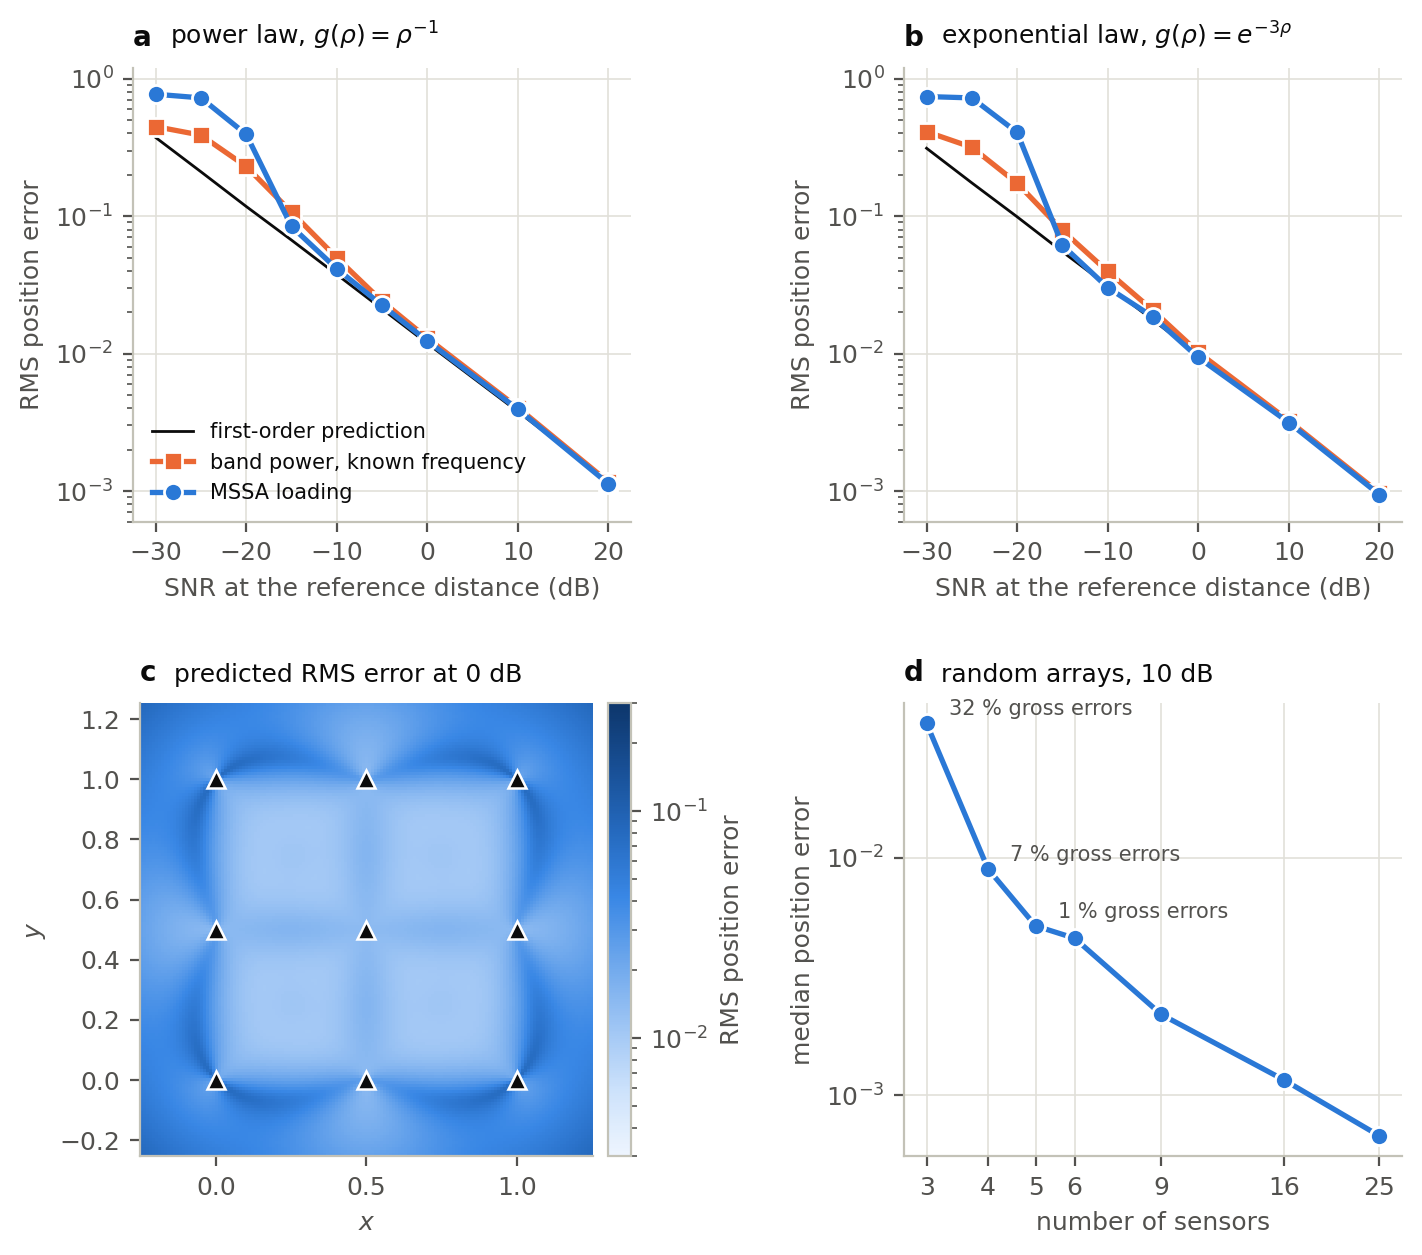
\includegraphics[width=0.88\textwidth]{fig2_accuracy.png}
    \caption{Accuracy for one source. (a, b) RMS position error against SNR for the MSSA loading and for band power at the known frequency, with the prediction of \eqref{eq:accuracy}, for the two attenuation laws. (c) Predicted RMS error over the plane at 0 dB for the grid of nine sensors (triangles); the error grows along circles that pass through neighbouring sensors, where the differential of the normalized map is close to singular (Theorem~\ref{thm:power-law}). (d) Median error against the number of sensors for random arrays at 10 dB, with the share of gross errors.}
    \label{fig:accuracy}
\end{figure}

\subsection{Two sources of different frequency}\label{sec:two-sources-of-different}

\emph{Strength.} Two sources at 10 and 13 Hz, at 10 dB, were localized from the loadings of Theorem~\ref{thm:loadings} and from pairs of singular vectors (Fig.~\ref{fig:two-sources}a). The former give a median error of 0.004--0.009 at every ratio of strengths, with no gross errors. The latter fail when the strengths are close: the median error is 0.34 with 97 \% gross errors at equal strength, 0.14 at a ratio of 1.05, 0.064 at 1.1 and 0.018 at 1.25, and the two methods coincide only from a ratio of 2. Singular vectors are a basis of the signal subspace, not a list of sources.

\emph{Frequency separation.} With equal strengths and a separation of half the Fourier resolution $1/T = 0.2$ Hz, both sources are localized with a median error of 0.008 at 10 dB and 0.003 at 20 dB, about twice the error at large separations (0.004 and 0.0013); at a quarter of the resolution the error is 0.025 and 0.008 (Fig.~\ref{fig:two-sources}b).

\emph{Position.} Two sources 3 Hz apart are localized equally well whether they are at one position or at different ones (0.0039 and 0.0041), and the same holds at a separation of one Fourier resolution. Closer than that, distinct fingerprints are what separates them: at a quarter of the resolution two sources at different positions are localized with a median error of 0.023, and two sources at one position are not separated at all (gross errors in 85 \% of trials).

\begin{figure}[tb]
\renewcommand{\figurename}{Fig.}
    \centering
    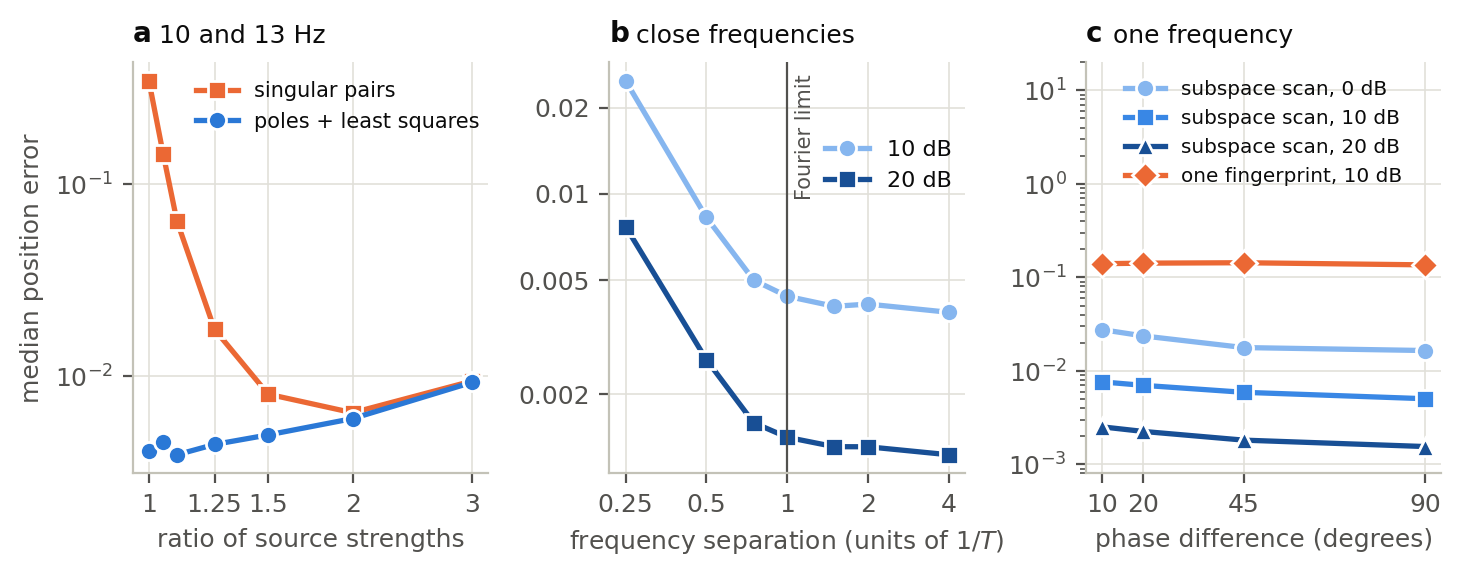
\includegraphics[width=1\textwidth]{fig3_two_sources.png}
    \caption{Two sources. (a) Different frequencies: median error of the worse-located source against the ratio of source strengths, for loadings from poles and least squares and for pairs of singular vectors. (b) Median error against the frequency separation in units of the Fourier resolution. (c) One frequency: subspace scan for two sources, and matching of a single fingerprint, against the phase difference.}
    \label{fig:two-sources}
\end{figure}

\subsection{Two sources of one frequency}\label{sec:two-sources-of-one}

For a single source the in-phase test at the 5 \% level rejects in 4.2, 4.3 and 5.5 \% of 1000 trials at 0, 10 and 20 dB, as it should. For two sources at 10 Hz it detects the second source in 83 \% of trials at a phase difference of 10$^{\circ}$ and 0 dB, in 98 \% at 20$^{\circ}$, and in all trials at larger phase differences or higher SNR. The subspace scan then localizes both sources with a median error of 0.016--0.028 at 0 dB, 0.005--0.008 at 10 dB and 0.0016--0.0025 at 20 dB, with gross errors in 1--3 \% of trials at 10 dB and above and in 2--13 \% at 0 dB (Fig.~\ref{fig:two-sources}c). Matching a single fingerprint to the same mode gives a position 0.14 away from the nearer source, whatever the SNR.

\subsection{Sensors and the attenuation law}\label{sec:sensors-and-the-attenuation}

\emph{Number of sensors.} For random arrays at 10 dB (Fig.~\ref{fig:accuracy}d; 20 arrays of each size, 30 sources each), three sensors give gross errors in 32 \% of trials: the second solution of Corollary~\ref{cor:sensors}(ii) lies inside $\Omega$ for part of the source positions. Four sensors give 7 \%, five 1 \%, and six or more none; four random sensors are never exactly on a circle but are often close to one. The median error falls from 0.009 with four sensors to 0.002 with nine and 0.0007 with twenty-five.

\emph{Attenuation exponent.} When the fit assumes an exponent different from the true $\gamma = 1$, the position is biased (Fig.~\ref{fig:models}a): at 0 dB the median error is 0.009 with the true exponent, 0.016--0.018 with an exponent wrong by 10 \%, 0.032--0.035 with one wrong by 20--25 \%, and 0.075--0.080 for exponents of 0.6 and 2. Estimating the exponent together with the position costs little: the median position error is 0.010, and the estimated exponent has a median of 1.00 and an interquartile range of 0.97--1.03.

\subsection{A dipolar source}\label{sec:a-dipolar-source}

A current dipole was placed in the upper half of a unit ball, at a distance of 0.3--0.7 from the centre, and its potential in a homogeneous conductor was recorded by 32 sensors on the upper hemisphere; the orientation was varied from radial to tangential (200 trials per point). The fit with the gain matrix of Section~\ref{sec:gain-matrix-models} localizes the dipole with a median error of 0.0006--0.0008 at 20 dB and 0.007 at 0 dB at every orientation (Fig.~\ref{fig:models}b). The distance-only law with $\gamma = 2$, fitted to the absolute loading, is in error by 0.21--0.26 of the radius at every orientation, including the radial one. A homogeneous conductor is the simplest volume conductor; a realistic head model changes the gain matrix and not the procedure.

\subsection{The complete procedure}\label{sec:the-complete-procedure}

\emph{Three sources with the rank estimated.} Three sources with frequencies between 5 and 30 Hz at least 2 Hz apart, amplitudes between 0.7 and 1.3 and mutual distances above 0.2 were processed by the algorithm of Section~\ref{sec:mssa-assisted-inverse-localization} with the calibrated threshold ($\kappa = 0.135$). The rank is correct in 97--98 \% of recordings from $-15$ dB to 20 dB, in 19 \% at $-20$ dB and never at $-25$ dB (Fig.~\ref{fig:models}c). When it is correct, the RMS position error equals the first-order prediction from $-5$ dB upward: 0.0215, 0.0128, 0.0039 and 0.0013 at $-5$, 0, 10 and 20 dB against 0.0221, 0.0124, 0.0040 and 0.0013 (Fig.~\ref{fig:models}d). At $-10$ dB it is 0.039 after exclusion of 2 \% gross errors, and at $-15$ dB a fifth of the positions are gross errors.

\emph{Rules for the number of components.} Table~\ref{tab:rank-rules} compares the thresholds of Section~\ref{sec:first-inverse-problem-estimating} on the same kind of recording. The uncorrected Marchenko--Pastur edge over-counts in a quarter to a third of recordings. The surrogate threshold is correct in every trial from $-5$ dB, and less often than the calibrated threshold at $-15$ dB.

\begin{table}[htb]
\centering
\caption{Three sources: probability of the correct rank (100 trials per row; 30 surrogates).}
\label{tab:rank-rules}
\begin{tabular}{l c c c}
\toprule
SNR$_0$ (dB) & calibrated threshold & edge without correction & surrogates \\
\midrule
$-15$ & 0.96 & 0.62 & 0.82 \\
$-5$ & 0.98 & 0.67 & 1.00 \\
$5$ & 0.96 & 0.64 & 1.00 \\
$20$ & 0.99 & 0.75 & 1.00 \\
\bottomrule
\end{tabular}
\end{table}

The surrogate threshold fails when sources differ in strength. For two sources at 10 and 17 Hz, the weaker having a mean SNR of $-6$ dB per sensor, the calibrated threshold returns rank 4 in 96--99 \% of 100 trials at each amplitude ratio from 1 to 100. The surrogate threshold does so at ratios of 1 and 3 and returns rank 2 in every trial at ratios of 10, 30 and 100: the surrogate spectrum inherits the power of the strong source and hides the weak one.

\begin{figure}[tb]
\renewcommand{\figurename}{Fig.}
    \centering
    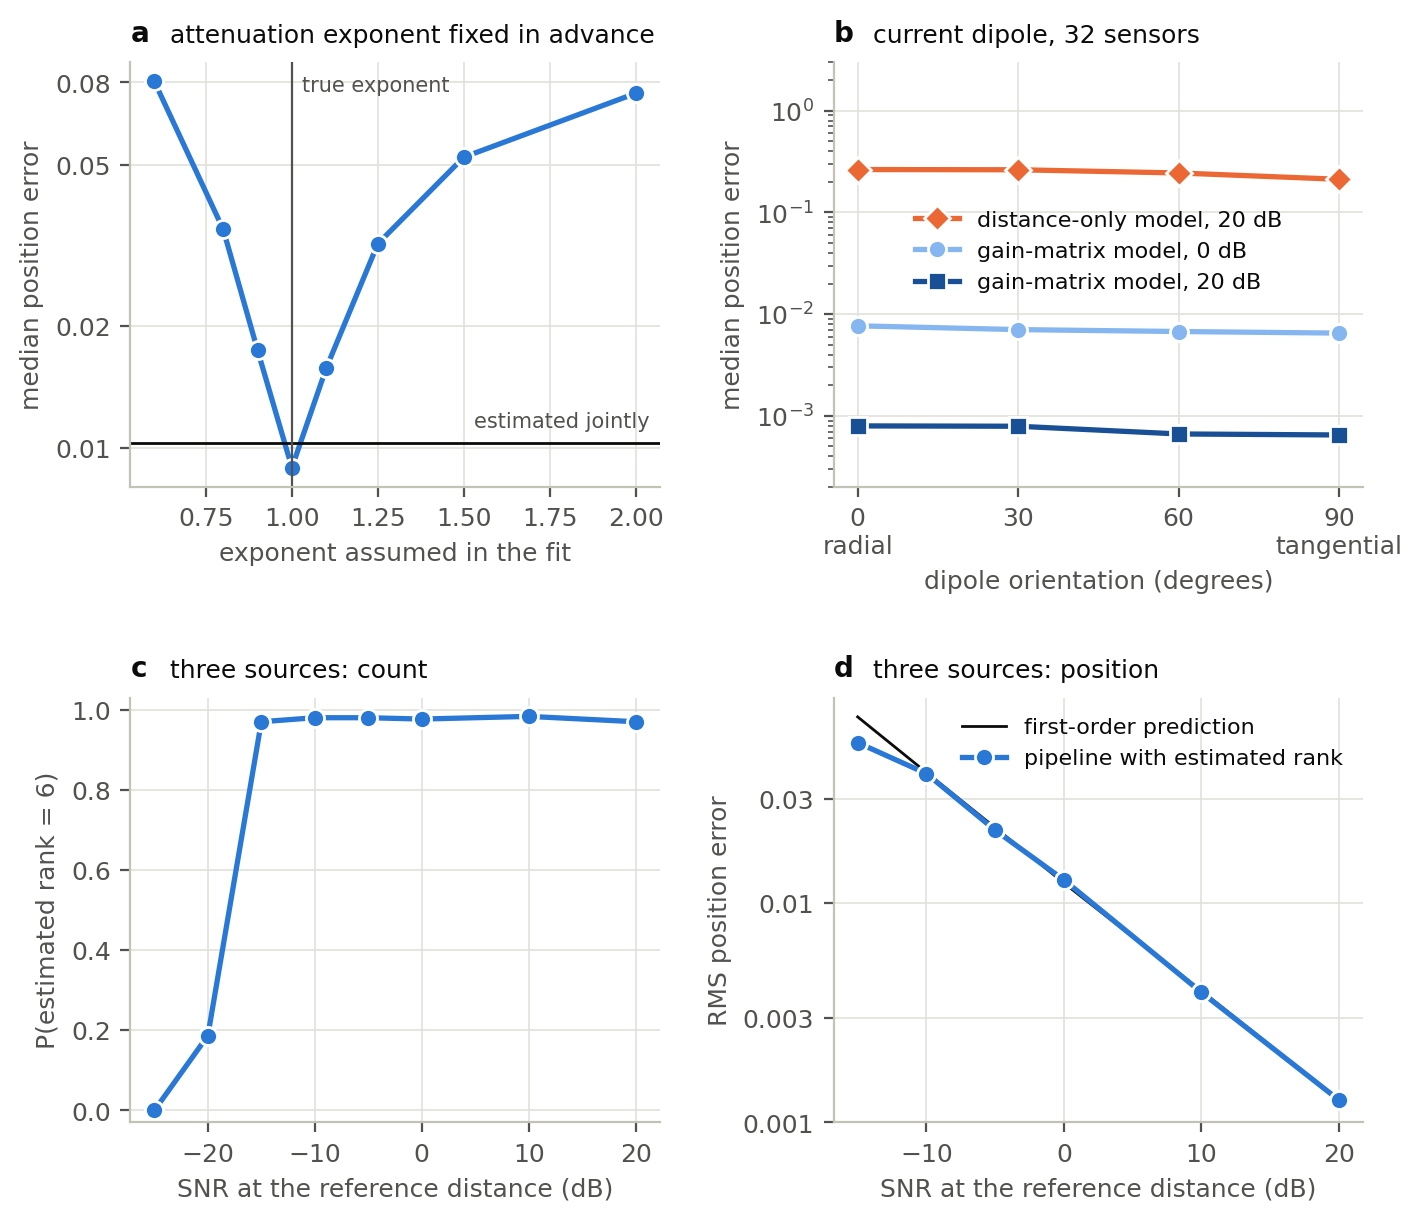
\includegraphics[width=0.88\textwidth]{fig4_models_pipeline.png}
    \caption{Models and the complete procedure. (a) Median position error when the attenuation exponent is fixed in advance at a value that may differ from the true one; the horizontal line is the error when the exponent is estimated together with the position. (b) Current dipole: gain-matrix model and distance-only model against the orientation of the dipole. (c) Three sources: probability that the estimated rank is correct. (d) Three sources: RMS position error of the procedure with estimated rank, and the prediction of \eqref{eq:accuracy}.}
    \label{fig:models}
\end{figure}

\subsection{Comparison with blind separation of independent components}\label{sec:comparison-with-blind-separation}

The count of \cite{ref-BernadotteBuchstaber, ref-Bernadotte05} concerns temporal modes; sources within one mode, or within one band, have to be separated in space. Blind methods do this from the statistics of the mixture: independent component analysis from its non-Gaussianity \cite{ref-Comon, ref-Hyvarinen}, second-order blind identification (SOBI) from its lagged covariances \cite{ref-Belouchrani}. Each spatial pattern they return can then be matched to an attenuation profile by \eqref{eq:matching}, as dipoles are fitted to component maps in EEG \cite{ref-Delorme}. We compared this route with the procedure of Section~\ref{sec:mssa-assisted-inverse-localization} on two sources of equal strength at different positions, at 10 dB (Table~\ref{tab:blind}). The blind methods were applied to the recording band-passed around the sources and were given the number of components. For sources of one band the plane of Section~\ref{sec:two-sources-in-one} was taken from the two leading spatial singular vectors of the recording band-passed between 8 and 12 Hz.

\begin{table}[htb]
\centering
\caption{Two sources at different positions: median position error, with the share of gross errors in parentheses (10 dB; 200 trials for 5 s, 100 for 200 s). The bursts and the Gaussian signals are narrow-band signals at 10 Hz.}
\label{tab:blind}
\begin{tabular}{l c c c}
\toprule
source signals and record length & this procedure & FastICA, then \eqref{eq:matching} & SOBI, then \eqref{eq:matching} \\
\midrule
sinusoids at 10 and 13 Hz, 5 s & 0.004 (0 \%) & 0.005 (1 \%) & 0.005 (0 \%) \\
10 Hz sinusoids in quadrature, 5 s & 0.007 (1 \%) & 0.115 (56 \%) & 0.111 (57 \%) \\
10 Hz sinusoids 20$^{\circ}$ apart, 5 s & 0.027 (3 \%) & 0.18 (92 \%) & 0.19 (92 \%) \\
independent bursts, 5 s & 0.007 (1 \%) & 0.12 (59 \%) & 0.16 (65 \%) \\
independent bursts, 200 s & 0.0011 (2 \%) & 0.021 (1 \%) & 0.16 (72 \%) \\
independent Gaussian signals, 5 s & 0.007 (0 \%) & 0.12 (59 \%) & 0.13 (65 \%) \\
independent Gaussian signals, 200 s & 0.0011 (1 \%) & 0.12 (59 \%) & 0.14 (61 \%) \\
\bottomrule
\end{tabular}
\end{table}

When the sources differ in frequency, the three routes agree. When they share a frequency, the blind methods fail on records of five seconds, whatever the signals. For sinusoids the failure is one of principle. Two sinusoids in quadrature trace a circle; every rotation of the pair has the same distribution and the same lagged covariances, and neither criterion can choose among the rotations. Sinusoids 20$^{\circ}$ apart have a correlation of 0.94, which contradicts independence. The scan localizes both pairs, because the forward model, and not a statistical criterion, selects the two directions within the plane.

For independent sources the blind methods are limited by the record: in five seconds two narrow-band signals of one band have a sample correlation of 0.15--0.4. With longer records independent component analysis improves for the non-Gaussian bursts, with gross errors in 45 \% of trials at 20 s, 19 \% at 60 s and 1 \% at 200 s, where its median error is still twenty times that of the scan (Fig.~\ref{fig:blind}). It does not improve for Gaussian sources, which it cannot separate in principle \cite{ref-Comon}. SOBI needs sources with different spectra \cite{ref-Belouchrani} and fails at every length. Blind separation also returns no more sources than there are sensors: of twelve sinusoids of different frequencies recorded by nine sensors, the modes of Section~\ref{sec:mssa-spatial-loading-as} locate all twelve within 0.05, and independent component analysis with nine components locates 39 \%.

Two remarks delimit the result. First, for sources that are not sinusoids the temporal decomposition contributes little to the spatial step. The trajectory matrix then has many modes in the band (a median rank of 19 for the bursts and of 10 for the Gaussian signals), and the plane obtained from their loadings gives larger errors than the plane of the band-passed recording, 0.015 and 0.011 against 0.007. Second, the blind methods keep two uses that the scan does not have. They need no forward model, and for independent non-Gaussian sources on long records they return the waveforms of sources that share a band (correlation 0.99 with the true waveforms at 200 s), which the temporal modes do not separate.

\begin{figure}[tb]
\renewcommand{\figurename}{Fig.}
    \centering
    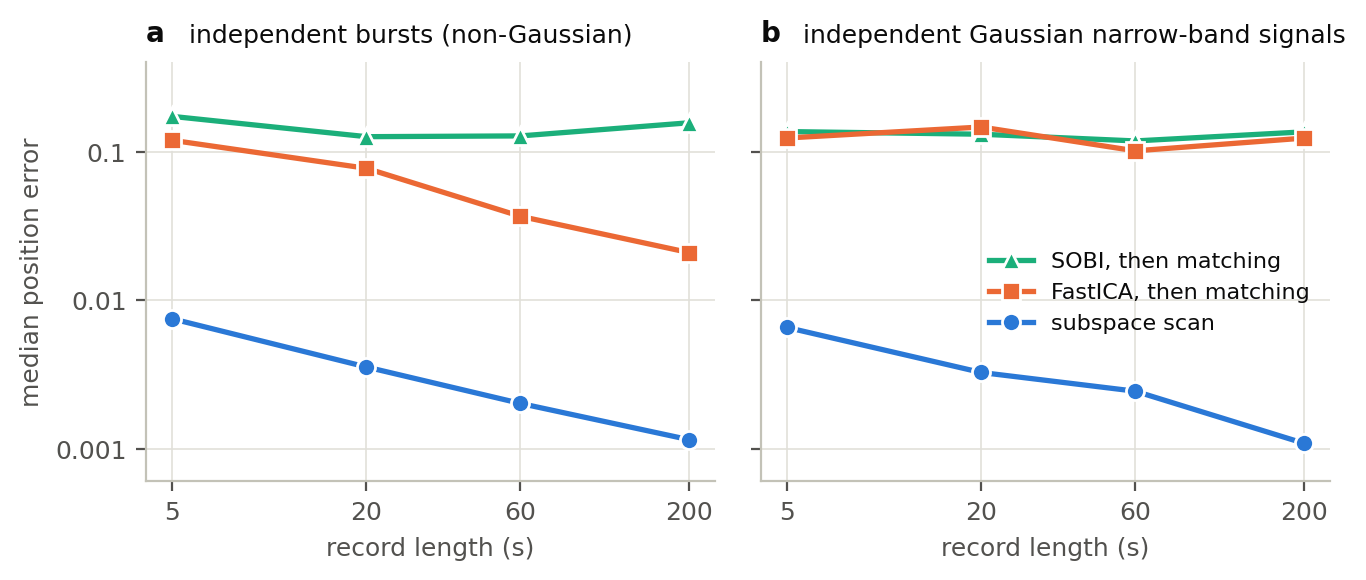
\includegraphics[width=0.88\textwidth]{fig5_blind_separation.png}
    \caption{Blind separation against record length: median position error for two independent sources of one band, located by the subspace scan and by blind separation followed by matching (10 dB). (a) Non-Gaussian bursts. (b) Gaussian narrow-band signals.}
    \label{fig:blind}
\end{figure}

\section{Applications}\label{sec:applications}

The method is general. It applies whenever multichannel observations are mixtures of latent oscillatory or quasi-oscillatory sources whose amplitudes attenuate across sensors, channels, features, or network positions. Like the source-number method of \cite{ref-BernadotteBuchstaber}, it is not tied to the brain, although EEG is where the framework was developed \cite{ref-BernadotteBuchstaber, ref-Bernadotte05, ref-Bernadotte10, ref-Bernadotte07, ref-Bernadotte06}.

\subsection{Neurophysiology and EEG/MEG}\label{sec:neurophysiology-and-eeg-meg}

In EEG/MEG, latent neural populations generate oscillatory activity recorded by multiple sensors. The attenuation profile is determined by distance, tissue conductivity, orientation, and lead-field geometry. It is therefore described by the gain-matrix model of Section~\ref{sec:forward-models-with-a} with the lead field of the head model, and not by a function of distance alone (Section~\ref{sec:a-dipolar-source}). MSSA can first estimate the number of active oscillatory modes \cite{ref-BernadotteBuchstaber, ref-Bernadotte05} and then provide spatial loading patterns for inverse source localization; the fit of Section~\ref{sec:gain-matrix-models} is the counterpart, for oscillatory modes, of fitting dipoles to the maps of independent components \cite{ref-Delorme}.

Potential uses include localization of alpha, beta, theta, or gamma generators; detection of pathological oscillatory sources; sleep-stage and coma-state analysis \cite{ref-Bernadotte07}; BCI calibration; and neurofeedback personalization.

\subsection{Wearable sensor networks}\label{sec:wearable-sensor-networks}

In wearable systems, physiological or mechanical oscillations may be recorded by distributed sensors. Examples include cardiac and respiratory oscillations, tremor, gait oscillations, muscle activation patterns, and biomechanical vibrations. If signal amplitude decays with distance or sensor coupling, MSSA-derived spatial loadings can identify the location of the latent oscillatory source on the body or device network. A lightweight real-time implementation of the Hankel embedding exists \cite{ref-Bernadotte06}.

\subsection{Industrial monitoring and predictive maintenance}\label{sec:industrial-monitoring-and-predictive}

Rotating machines, turbines, engines, and mechanical structures often generate oscillations that propagate through a sensor network with attenuation. MSSA can separate latent vibration modes, estimate their number \cite{ref-BernadotteBuchstaber}, and localize their origin. Applications include fault localization, bearing defect detection, turbine vibration analysis, structural health monitoring, and acoustic emission localization.

\subsection{Seismology and geophysics}\label{sec:seismology-and-geophysics}

Seismic or geophysical events generate waves recorded by spatially distributed sensors. When amplitude attenuation is known or calibrated, MSSA can separate oscillatory components, count them as in \cite{ref-BernadotteBuchstaber}, and use spatial loading profiles for source localization. Possible uses include microseismic event localization, volcanic tremor analysis, underground structural monitoring, and oceanographic oscillation source detection. Surface arrays are planar, the case of Corollary~\ref{cor:sensors}(iv).

\subsection{Wireless and electromagnetic systems}\label{sec:wireless-and-electromagnetic-systems}

In wireless sensor networks, oscillatory signals may be emitted by latent sources and recorded with power decay across receivers; their number is estimated as in \cite{ref-BernadotteBuchstaber}. The MSSA attenuation-fingerprint framework can support emitter localization, interference source detection, spectrum monitoring, and distributed antenna diagnostics.

\subsection{Financial sector}\label{sec:financial-sector}

The financial sector is less obviously spatial, but the same mathematical structure applies if coordinates are interpreted as positions in a latent market-factor space rather than physical space.

Financial markets produce multichannel time series where channels may be asset returns, sector indices, volatility curves, yield-curve points, liquidity indicators, order-book features, macroeconomic indicators, or cross-market spreads. Latent oscillatory sources may represent business-cycle components, liquidity cycles, volatility regimes, sector rotation waves, risk-on/risk-off oscillations, intraday microstructure cycles, or hidden market stress modes.

Factor analysis of economic data has been formulated as an extremal problem on Grassmann manifolds \cite{ref-BuchstaberMaslov}, the geometry that underlies the unfolding of time series \cite{ref-Buchstaber}. The analogue of physical attenuation is factor-exposure decay across a feature space. A latent financial oscillator may affect some assets strongly and others weakly depending on their distance from the source in a financial similarity space. For example, coordinates $p_j$ may be assigned to assets or indicators in a latent embedding space constructed from sector membership, correlation distance, factor loadings, duration, maturity, liquidity, geography, market capitalization, or volatility-regime similarity.

A latent financial source at coordinate $q_k$ produces an oscillatory component with exposure \[
a_{jk} = \alpha_k\, g(d(p_j, q_k)),
\] where $d(p_j, q_k)$ is a financial distance and $g$ is an exposure-decay function. MSSA extracts latent oscillatory market modes $s_k(t)$ and their loadings $\widehat{a}_k$ across assets. The loading vector becomes an amplitude fingerprint of the latent financial source. Matching this fingerprint to candidate points in the financial feature space, by \eqref{eq:matching} with the profiles $g_q = (g(d(p_1, q)), \dots, g(d(p_m, q)))^{\top}$, can localize the source of the regime.

Two of the conditions of Section~\ref{sec:conditions-required-for-coordinate} need attention in this setting. The coordinates $p_j$ must be known independently of the loadings that are to be explained: an embedding constructed from the correlations of the same series is not independent of them, and matching against it is circular. Coordinates that exist beforehand satisfy the condition directly --- maturity along a yield curve, strike and maturity on a volatility surface, the geographical position of regional indices. And the exposure-decay function is not given by physics. It has to be chosen as a parametric family whose parameters are estimated together with the position, as the exponent is in Section~\ref{sec:sensors-and-the-attenuation}, and the residual fraction of Section~\ref{sec:one-source-per-mode} shows whether the family fits. On a yield curve, for example, the channels are yields at maturities $p_1 < \dots < p_m$, $d = 1$, and an oscillatory component with exposure $\alpha\, g(|p_j - q|)$ is located at a maturity $q$; three or more maturities determine $q$ uniquely for a power law (Theorem~\ref{thm:power-law} with $d = 1$).

Potential financial applications include hidden risk-factor localization, sector-rotation detection, volatility-regime mapping, yield-curve dynamics, market-contagion analysis, and portfolio risk decomposition.

\section{Discussion}\label{sec:discussion}

This article formulates MSSA as a general method for solving two linked inverse problems in multichannel oscillatory systems. The first inverse problem is the recovery of the number of latent oscillatory sources. This problem was previously addressed in Bernadotte's Hankel-embedding framework \cite{ref-BernadotteBuchstaber, ref-Bernadotte05}, where the effective rank of time-series unfoldings was used to estimate the number of active oscillators. MSSA generalizes this idea to multichannel block-Hankel embeddings.

The second inverse problem is the recovery of source coordinates. This becomes possible when each latent oscillatory source is observed with distance-dependent amplitude attenuation. In that case, the spatial loading vector recovered by MSSA is not merely a statistical component. It is an empirical amplitude fingerprint of the source location.

The coordinate recovery problem then reduces to matching this empirical fingerprint to a theoretical attenuation profile generated by candidate coordinates. The solution is unique when the normalized attenuation map is injective, the sensor geometry is non-degenerate, sources are temporally separable, spatial fingerprints are distinguishable where that is needed, and noise is sufficiently small. Sections~\ref{sec:identifiability} and \ref{sec:conditions-required-for-coordinate} turn each of these conditions into a statement that can be checked for a given array, law and recording.

This framework separates the inverse problem into two stages: \[
X \xrightarrow{\ \mathrm{MSSA}\ } (\widehat{r}, \widehat{a}_k, \widehat{s}_k) \xrightarrow{\ \text{attenuation matching}\ } \widehat{q}_k .
\] The first stage is structural. It identifies how many oscillatory sources are present and extracts their temporal modes and spatial loadings. The second stage is geometric. It maps spatial loadings to source coordinates using an attenuation model.

This separation is useful because the full inverse problem is typically ill-conditioned. MSSA regularizes it by reducing the raw multichannel signal to a finite set of coherent oscillatory components before spatial localization is attempted. The experiments locate the benefit. For one source the reduction changes little, and any amplitude fingerprint attains the accuracy that the geometry permits. With several sources it is what makes the problem separable: each source is fitted alone, in $d$ unknowns, whatever the strengths of the others, and their number is decided beforehand.

The central methodological claim is:

\begin{quote}
Multichannel Singular Spectrum Analysis converts a multichannel time series into a finite set of latent oscillatory modes. When the sources of these modes undergo amplitude attenuation across sensors, the MSSA spatial loading vector becomes an amplitude fingerprint of the source coordinate. Under known attenuation law, known sensor geometry, and injective source-to-sensor mapping, source coordinates are identifiable from these fingerprints.
\end{quote}

In formula form, $X \xrightarrow{\ \mathrm{MSSA}\ } \widehat{a}_k \approx \alpha_k\, g_{q_k}$, and therefore $\widehat{q}_k$ is given by \eqref{eq:matching}. This is the bridge between MSSA, source-number estimation, and coordinate recovery for attenuating oscillatory systems.

The scope of the present results is as follows. All experiments are simulations with white sensor noise that is independent between channels and of equal variance; a coloured or spatially correlated background, as in EEG, requires whitening before the count and reduces the gain from pooling channels. The forward model is instantaneous: propagation delays would add a phase to the loadings, which carries further information about position and is not used here. The attenuation law must be known up to a few parameters. Sources of one frequency and damping are resolved only two at a time, and not at all when they are in phase. Blind separation of independent components remains the tool when no forward model is available, or when the waveforms of sources that share a band are wanted (Section~\ref{sec:comparison-with-blind-separation}). Validation on recordings with known source positions is the next step.

The method is not limited to EEG or BCI. It applies to any domain where latent oscillatory sources are observed through multiple channels with distance-dependent or similarity-dependent attenuation. This includes neurophysiology, wearable sensors, industrial monitoring, geophysics, wireless systems, and financial markets.

\appendix

\section{Calibration of the rank threshold}\label{app:calibration-of-the}

In \cite{ref-BernadotteBuchstaber, ref-Bernadotte05} the number of components is read from the effective rank, or $\varepsilon$-rank, of the unfolding. The threshold of Section~\ref{sec:first-inverse-problem-estimating} fixes that rank against a white noise floor. It was studied on white-noise recordings, for which the estimated rank should be zero. With $\kappa = 0$ a non-zero rank is returned for 16--29 \% of trajectory matrices at $L = 10$, 37--52 \% at $L = 40$ and 64--80 \% at $L = 80$, against 13--23 \% for matrices of the same shape with independent entries. The correction that restores a 5 \% rate grows with the window, falls with the record length and falls slowly with the number of channels (Table~\ref{tab:kappa}); over 29 configurations it is described by \[
\kappa_{95} \approx 0.44\; L^{0.71}\, K^{-0.52}\, m^{-0.22}
\] with $R^2 = 0.97$ on a logarithmic scale. Simulation for the configuration at hand is the exact method; for $m = 9$, $N = 500$, $L = 40$ it gives 0.12--0.14.

\begin{table}[htb]
\centering
\caption{Correction $\kappa_{95}$ for a 5 \% false-positive rate on white noise.}
\label{tab:kappa}
\begin{tabular}{l c c c c}
\toprule
 & $L = 10$ & $L = 20$ & $L = 40$ & $L = 80$ \\
\midrule
$N = 1000$, $m = 1$ & 0.055 & 0.102 & 0.171 & 0.231 \\
$N = 1000$, $m = 8$ & 0.038 & 0.075 & 0.112 & 0.178 \\
$N = 4000$, $m = 1$ & 0.027 & 0.042 & 0.072 & 0.125 \\
$N = 4000$, $m = 8$ & 0.015 & 0.031 & 0.056 & 0.080 \\
\bottomrule
\end{tabular}
\end{table}

With the calibrated correction the rank of three oscillators shared by all channels is recovered in 93--99 \% of trials from $-5$ dB per channel upward for one channel, from $-7.5$ dB for two and from $-12.5$ dB for eight. Coloured noise breaks the calibration: first-order autoregressive noise with coefficient 0.3 already yields a mean rank of 11 on noise alone. Whitening every channel by a running median of its periodogram, which ignores narrow peaks, restores the null for coefficients up to 0.9 at the price of a larger correction; steeper backgrounds call for a null that carries their colour \cite{ref-Allen}.

\section{Joint and channel-wise analysis}\label{app:joint-and-channel}

In \cite{ref-Bernadotte05} every trace is embedded separately. Section~\ref{sec:block-hankel-mssa-matrix} states that joint decomposition reveals components that single channels do not. Table~\ref{tab:joint} gives the size of the effect and its limit, for eight channels, $N = 1000$, $L = 50$ and white noise, with channel-wise SSA and joint MSSA applied to the same recordings and the rank estimated by the calibrated threshold. The gain belongs to shared structure: it is close to its upper bound of $10 \log_{10} m$ dB when all channels carry the same oscillators, small when only part of the structure is shared, and negative when the channels have nothing in common, in agreement with \cite{ref-Golyandina03}. In the localization problem all sensors record every source, which is the favourable case.

\begin{table}[htb]
\centering
\caption{Channel-wise SSA and joint MSSA on the same eight-channel recordings.}
\label{tab:joint}
\begin{tabular}{p{0.6\textwidth} c c}
\toprule
 & channel-wise SSA & joint MSSA \\
\midrule
output SNR at 0 dB input, three oscillators shared by all channels & 10.7 dB & 17.9 dB \\
the same, two shared oscillators and one private to each channel & 10.7 dB & 12.6 dB \\
the same, three private oscillators in each channel & 10.7 dB & 8.8 dB \\
detection of an oscillation common to all channels, $-17.5$ dB & 11 \% & 96 \% \\
detection of an oscillation present in one channel, $-12.5$ dB & 89 \% & 51 \% \\
\bottomrule
\end{tabular}
\end{table}

\section*{Code and data availability}\label{code-and-data-availability}

The embedding, the decomposition and the rank estimate use the \texttt{aicumene-mssa} package (\url{https://github.com/aicumene/MSSA}). Pole estimation, loading extraction, the tests and the matching are in \texttt{paper/experiments/loc\_common.py} of the same repository, together with the scripts and numerical results of Section~\ref{sec:numerical-experiments}. No experimental data were used.


\renewcommand{\refname}{REFERENCES}
 \begin{thebibliography}{0}

\bibitem{ref-BernadotteBuchstaber} Alexandra Bernadotte, Victor Buchstaber. ``Method for Evaluating the Number of Signal Sources and Application to Non-invasive Brain-computer Interface.'' arXiv preprint arXiv:2410.11844. 2024.

\bibitem{ref-Bernadotte05} Alexandra Bernadotte. ``Estimating the Number of Sources in EEG with Hankel Embedding for Brain-computer Interface.'' 12th International Conference on Automation, Robotics, and Applications. IEEE. 2026. pp 621-626. doi: 10.1109/ICARA69401.2026.11480398

\bibitem{ref-Buchstaber} V. M. Buchstaber. ``Time Series Analysis and Grassmannians.''  Applied problems of Radon transform, Amer. Math. Soc. Transl. 1994. Vol 2 (162), pages 1--17.

\bibitem{ref-BuchstaberMaslov} V. M. Buchstaber, V. K. Maslov. ``Factor Analysis and Extremal Problems on Grassmann Manifolds.'' Mathematical Methods for Solving Economic Problems. 1977. Vol 7, pp. 85--102.

\bibitem{ref-Bernadotte10} Alexandra Bernadotte.  ``Topology-driven classification of time series.'' bioRxiv 2026.04.25.720787. 2026. doi:  10.64898/2026.04.25.720787

\bibitem{ref-Bernadotte07} Alexandra Bernadotte, Ivan Menshikov. ``Brain Oscillator Intrinsic Dimension marks consciousness, recovery mode, and failed downshifting in coma.'' Aicumene. Preprint. 2026. DOI: 10.13140/RG.2.2.31610.25288 Available: \url{https://research.aicumene.com/papers/boid-coma/}

\bibitem{ref-Bernadotte06} Ivan Menshikov, Nikita Elfimov, Alexandra Bernadotte.  ``A Lightweight Hankel-Embedded Pipeline for Real-Time EEG Filtering and Classification.''  12th International Conference on Automation, Robotics, and Applications. IEEE. 2026. pp 589-593. doi: 10.1109/ICARA69401.2026.11480292

\bibitem{ref-BernadotteAutomata} Bernadotte A. ``Structural Modification of the Finite State Machine to Solve the Exponential Explosion Problem.'' Programmnaya Ingeneria. 2022. Vol 13(9), pp. 449--461. doi: 10.17587/prin.13.449-461

\bibitem{ref-Broomhead} Broomhead D. S., King G. P. ``Extracting qualitative dynamics from experimental data.'' Physica D. 1986. Vol 20, pp. 217--236.

\bibitem{ref-Vautard} Vautard R., Ghil M. ``Singular spectrum analysis in nonlinear dynamics, with applications to paleoclimatic time series.'' Physica D. 1989. Vol 35, pp. 395--424.

\bibitem{ref-Golyandina01} Golyandina N., Nekrutkin V., Zhigljavsky A. ``Analysis of Time Series Structure: SSA and Related Techniques.'' Chapman \& Hall/CRC. 2001.

\bibitem{ref-Golyandina02} Golyandina N., Zhigljavsky A. ``Singular Spectrum Analysis for Time Series.'' Springer. 2013.

\bibitem{ref-Golyandina03} Golyandina N., Korobeynikov A., Shlemov A., Usevich K. ``Multivariate and 2D extensions of singular spectrum analysis with the Rssa package.'' Journal of Statistical Software. 2015. Vol 67(2), pp. 1--78.

\bibitem{ref-Plaut} Plaut G., Vautard R. ``Spells of low-frequency oscillations and weather regimes in the Northern Hemisphere.'' Journal of the Atmospheric Sciences. 1994. Vol 51, pp. 210--236.

\bibitem{ref-Wax} Wax M., Kailath T. ``Detection of signals by information theoretic criteria.'' IEEE Transactions on Acoustics, Speech, and Signal Processing. 1985. Vol 33, pp. 387--392.

\bibitem{ref-Kritchman} Kritchman S., Nadler B. ``Non-parametric detection of the number of signals: hypothesis testing and random matrix theory.'' IEEE Transactions on Signal Processing. 2009. Vol 57, pp. 3930--3941.

\bibitem{ref-Schmidt} Schmidt R. O. ``Multiple emitter location and signal parameter estimation.'' IEEE Transactions on Antennas and Propagation. 1986. Vol 34, pp. 276--280.

\bibitem{ref-Roy} Roy R., Kailath T. ``ESPRIT --- estimation of signal parameters via rotational invariance techniques.'' IEEE Transactions on Acoustics, Speech, and Signal Processing. 1989. Vol 37, pp. 984--995.

\bibitem{ref-Li} Li D., Hu Y. H. ``Energy-based collaborative source localization using acoustic microsensor array.'' EURASIP Journal on Advances in Signal Processing. 2003. Vol 2003, 985029.

\bibitem{ref-Sheng} Sheng X., Hu Y. H. ``Maximum likelihood multiple-source localization using acoustic energy measurements with wireless sensor networks.'' IEEE Transactions on Signal Processing. 2005. Vol 53, pp. 44--53.

\bibitem{ref-Meng} Meng W., Xiao W. ``Energy-based acoustic source localization methods: a survey.'' Sensors. 2017. Vol 17, 376.

\bibitem{ref-Ho} Ho K. C., Sun M. ``Passive source localization using time differences of arrival and gain ratios of arrival.'' IEEE Transactions on Signal Processing. 2008. Vol 56, pp. 464--477.

\bibitem{ref-Patwari} Patwari N., Ash J. N., Kyperountas S., Hero A. O., Moses R. L., Correal N. S. ``Locating the nodes: cooperative localization in wireless sensor networks.'' IEEE Signal Processing Magazine. 2005. Vol 22(4), pp. 54--69.

\bibitem{ref-Mosher01} Mosher J. C., Lewis P. S., Leahy R. M. ``Multiple dipole modeling and localization from spatio-temporal MEG data.'' IEEE Transactions on Biomedical Engineering. 1992. Vol 39, pp. 541--557.

\bibitem{ref-Delorme} Delorme A., Palmer J., Onton J., Oostenveld R., Makeig S. ``Independent EEG sources are dipolar.'' PLoS ONE. 2012. Vol 7, e30135.

\bibitem{ref-Comon} Comon P. ``Independent component analysis, a new concept?'' Signal Processing. 1994. Vol 36, pp. 287--314.

\bibitem{ref-Hyvarinen} Hyv\"arinen A., Oja E. ``Independent component analysis: algorithms and applications.'' Neural Networks. 2000. Vol 13, pp. 411--430.

\bibitem{ref-Belouchrani} Belouchrani A., Abed-Meraim K., Cardoso J. F., Moulines E. ``A blind source separation technique using second-order statistics.'' IEEE Transactions on Signal Processing. 1997. Vol 45, pp. 434--444.

\bibitem{ref-Fliess} Fliess M. ``Matrices de Hankel.'' Journal de Math\'ematiques Pures et Appliqu\'ees. 1974. Vol 53, pp. 197--222.

\bibitem{ref-Marchenko} Marchenko V. A., Pastur L. A. ``Distribution of eigenvalues for some sets of random matrices.'' Mathematics of the USSR-Sbornik. 1967. Vol 1, pp. 457--483.

\bibitem{ref-Yin} Yin Y. Q., Bai Z. D., Krishnaiah P. R. ``On the limit of the largest eigenvalue of the large dimensional sample covariance matrix.'' Probability Theory and Related Fields. 1988. Vol 78, pp. 509--521.

\bibitem{ref-Johnstone} Johnstone I. M. ``On the distribution of the largest eigenvalue in principal components analysis.'' Annals of Statistics. 2001. Vol 29, pp. 295--327.

\bibitem{ref-Bryc} Bryc W., Dembo A., Jiang T. ``Spectral measure of large random Hankel, Markov and Toeplitz matrices.'' Annals of Probability. 2006. Vol 34, pp. 1--38.

\bibitem{ref-Allen} Allen M. R., Smith L. A. ``Monte Carlo SSA: detecting irregular oscillations in the presence of colored noise.'' Journal of Climate. 1996. Vol 9, pp. 3373--3404.

\bibitem{ref-Golyandina04} Golyandina N., Shlemov A. ``Variations of singular spectrum analysis for separability improvement: non-orthogonal decompositions of time series.'' Statistics and Its Interface. 2015. Vol 8, pp. 277--294.

\bibitem{ref-Hua} Hua Y., Sarkar T. K. ``Matrix pencil method for estimating parameters of exponentially damped/undamped sinusoids in noise.'' IEEE Transactions on Acoustics, Speech, and Signal Processing. 1990. Vol 38, pp. 814--824.

\bibitem{ref-Rife} Rife D. C., Boorstyn R. R. ``Single-tone parameter estimation from discrete-time observations.'' IEEE Transactions on Information Theory. 1974. Vol 20, pp. 591--598.

\bibitem{ref-Mosher02} Mosher J. C., Leahy R. M., Lewis P. S. ``EEG and MEG: forward solutions for inverse methods.'' IEEE Transactions on Biomedical Engineering. 1999. Vol 46, pp. 245--259.

\bibitem{ref-Baillet} Baillet S., Mosher J. C., Leahy R. M. ``Electromagnetic brain mapping.'' IEEE Signal Processing Magazine. 2001. Vol 18(6), pp. 14--30.

\bibitem{ref-Coxeter} Coxeter H. S. M., Greitzer S. L. ``Geometry Revisited.'' Mathematical Association of America. 1967.

\bibitem{ref-Chan} Chan Y. T., Ho K. C. ``A simple and efficient estimator for hyperbolic location.'' IEEE Transactions on Signal Processing. 1994. Vol 42, pp. 1905--1915.

\bibitem{ref-Torrieri} Torrieri D. J. ``Statistical theory of passive location systems.'' IEEE Transactions on Aerospace and Electronic Systems. 1984. Vol 20, pp. 183--198.

 \end{thebibliography}


\end{document}
